%%% TeX-command-extra-options: "-shell-escape"
\documentclass{llncs}
% \documentclass[llncs, a4paper, UKenglish, cleveref, autoref, thm-restate]{article}
\usepackage[utf8]{inputenc} % Required for inputting international characters
\usepackage[T1]{fontenc} % Output font encoding for international characters
% \usepackage[backend=bibtex,style=alphabetic,natbib=true]{biblatex}
% \usepackage[backend=bibtex,style=alphabetic,natbib=true]{biblatex}
% \addbibresource{references.bib}
\pagestyle{plain}

\usepackage{amsmath, mathpartir, stmaryrd}
%, amssymb, amsfonts, stmaryrd}
% \usepackage{mathpartir}
% \usepackage{bussproofs}

\usepackage{caption}
\usepackage{subcaption}
\usepackage{graphicx}
\usepackage{enumitem}
\usepackage{xparse}
\usepackage[usenames, dvipsnames]{xcolor}
\usepackage{lipsum}
\usepackage{xargs}
\usepackage{hyperref}
\usepackage{tikz-cd}
\usepackage{todonotes}
\usepackage{url}
\usepackage{xspace}
\usepackage{rotating}
\usepackage{quiver}
\usepackage{minted}
\usepackage{newunicodechar}
\usepackage{microtype}
% \addbibresource{references.bib}
\usepackage{array}   % for \newcolumntype macro
\newcolumntype{C}{>{$}c<{$}} % math-mode version of "l" column type
\newcolumntype{L}{>{$}l<{$}} % math-mode version of "l" column type

\usepackage{inconsolata}
% \usepackage{draftwatermark}
% \SetWatermarkText{Confidential}
% \SetWatermarkScale{4}
% \SetWatermarkColor[gray]{0.9}

\hypersetup{
  linktocpage,
  colorlinks,
  citecolor=BlueViolet,
  filecolor=red,
  linkcolor=Blue,
  urlcolor=BrickRed
}
\newcommand{\mpav}[1]{\textcolor{red}{\textsc{Marco}: #1}}
\newcommand{\dcas}[1]{\textcolor{ForestGreen}{\textsc{David}: #1}}
\newcommand{\mvol}[1]{\textcolor{blue}{\textsc{Michael}: #1}}
% \newcommand{\proofcomment}[1]{\text{\{ #1 \}}}
% \newenvironment{proofof}[1] {\begin{proof}[Proof of {#1}]}{\end{proof}}
\newcommand{\eqdef}{\stackrel{\mathrm{\Delta}}{=}}
\newcommand{\eqiff}{\stackrel{\triangle}{\iff}}
\newcommand{\bnfeq}{\mathrel{::=}}
\newcommand{\defeq}{\triangleq}
\newcommand{\rul}[3]{\frac{#2}{#3}\;  {\textrulelabel{#1}}}
\newcommand{\den}[1]{\llbracket #1 \rrbracket}
\newcommand{\jud}[3]{#1 \vdash #2 : #3}
\newcommand{\bden}[1]{\llparenthesis#1 \rrparenthesis}
\newcommand{\bigslant}[2]{{\raisebox{.2em}{$#1$}\left/\raisebox{-.2em}{$#2$}\right.}}
\newcommand{\quotient}[2]{\bigslant{#1}{#2}}
\newcommand{\curry}{\Lambda}
\newcommand{\uncurry}{\begin{sideways}\begin{sideways}$\Lambda$\end{sideways}\end{sideways}}
\newcommand{\Bool}{\mathbb{B}}
\newcommand{\N}{\mathbb{N}}
\newcommand{\Nat}{\N}
\newcommand{\R}{\mathbb{R}}
\newcommand{\Sets}{\mathbf{Set}}
\newcommand{\blacklater}{\blacktriangleright}
\newcommand{\tot}{\mathcal{S}}
\newcommand{\PSh}{\ensuremath{\textbf{PSh}(\omega)}}

\newsavebox{\lbananabox}
\newcommand{\lbananamacro}{%
  
\begin{tikzpicture}[baseline=0.25em,xscale=0.005em,yscale=0.005em]
  \draw[solid, join=round] (2,0) to[out=140,in=-90] (0,3) to[out=90,in=-140] (2,6) -- (2.1,5.9)
              to[out=-120,in=90] (1.2,3) to[out=-90,in=120] (2.1,0.1) -- cycle;
\end{tikzpicture}
}
\savebox{\lbananabox}{\lbananamacro}
\newcommand{\lbanana}{\mathopen{\usebox{\lbananabox}\hspace{-0.6ex}}}


\newsavebox{\rbananabox}
\newcommand{\rbananamacro}{%
  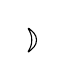
\begin{tikzpicture}[baseline=0.25em,xscale=-0.005em,yscale=0.005em]
  \draw[solid, join=round] (2,0) to[out=140,in=-90] (0,3) to[out=90,in=-140] (2,6) -- (2.1,5.9)
              to[out=-120,in=90] (1.2,3) to[out=-90,in=120] (2.1,0.1) -- cycle;
  \end{tikzpicture}
}
\savebox{\rbananabox}{\rbananamacro}
\newcommand{\rbanana}{\mathclose{\usebox{\rbananabox}}}


\newsavebox{\lbansbox}
\newcommand{\lbansmacro}{%
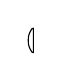
\begin{tikzpicture}[baseline=0.45ex,xscale=0.006em,yscale=0.012ex]%
% curvey bananas
%\draw[solid,join=round,fill=yellow] (2,0) to[out=140,in=-90] (0,3) to[out=90,in=-140] (2,6) -- (2.1,5.9) to[out=-120,in=90] (1.2,3) to[out=-90,in=120] (2.1,0.1) -- cycle;%
% fitted lenses
\draw[solid,join=round] (1.8,6) -- (1.5,5.9) to[out=-120, in=90] (0.7,3) to[out=-90, in=120] (1.5,0.1) -- (1.8,0) -- cycle;%
\end{tikzpicture}}
\savebox{\lbansbox}{\lbansmacro}
\newcommand{\lbans}{\mathopen{\usebox{\lbansbox}\mspace{1mu}}}

\newsavebox{\rbansbox}
\newcommand{\rbansmacro}{%
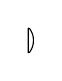
\begin{tikzpicture}[baseline=0.45ex,xscale=-0.006em,yscale=0.012ex]%
% curvey bananas
%\draw[solid,join=round,fill=yellow] (2,0) to[out=140,in=-90] (0,3) to[out=90,in=-140] (2,6) -- (2.1,5.9) to[out=-120,in=90] (1.2,3) to[out=-90,in=120] (2.1,0.1) -- cycle;%
% fitted lenses
\draw[solid,join=round] (1.8,6) -- (1.5,5.9) to[out=-120, in=90] (0.7,3) to[out=-90, in=120] (1.5,0.1) -- (1.8,0) -- cycle;%
\end{tikzpicture}}
\savebox{\rbansbox}{\rbansmacro}
\newcommand{\rbans}{\mathclose{\mspace{1mu}\usebox{\rbansbox}}}

\newsavebox{\llensbox}
\newcommand{\llensmacro}{%
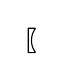
\begin{tikzpicture}[baseline=0.45ex,xscale=0.006em,yscale=0.012ex]%
\draw[solid,join=round] (1.4,0) -- (0,0) -- (0,6) -- (1.4,6) -- (1.5,5.9) to[out=-120, in=90] (0.7,3) to[out=-90, in=120] (1.5,0.1) -- cycle;%
\end{tikzpicture}}
\savebox{\llensbox}{\llensmacro}
\newcommand{\llens}{\mathopen{\usebox{\llensbox}\mspace{1mu}}}

\newsavebox{\rlensbox}
\newcommand{\rlensmacro}{%
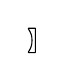
\begin{tikzpicture}[baseline=0.45ex,xscale=-0.006em,yscale=0.012ex]%
\draw[solid,join=round] (1.4,0) -- (0,0) -- (0,6) -- (1.4,6) -- (1.5,5.9) to[out=-120, in=90] (0.7,3) to[out=-90, in=120] (1.5,0.1) -- cycle;%
\end{tikzpicture}}
\savebox{\rlensbox}{\rlensmacro}
\newcommand{\rlens}{\mathclose{\mspace{1mu}\usebox{\rlensbox}}}

% filled versions
\newcommand{\Lbanana}{%
  \mathopen{\mspace{1mu}\tikz[baseline=0.25em,xscale=0.006em,yscale=0.006em]
  \fill (2,0) to[out=140,in=-90] (0,3) to[out=90,in=-140] (2,6) -- (2.1,5.9)
              to[out=-120,in=90] (1.2,3) to[out=-90,in=120] (2.1,0.1) -- cycle;\mspace{1mu}}}
\newcommand{\Rbanana}{%
  \mathclose{\mspace{1mu}\tikz[baseline=0.25em,xscale=-0.006em,yscale=0.006em]
  \fill (2,0) to[out=140,in=-90] (0,3) to[out=90,in=-140] (2,6) -- (2.1,5.9)
              to[out=-120,in=90] (1.2,3) to[out=-90,in=120] (2.1,0.1) -- cycle;}}
% % lens brackets (using TikZ)
% \newcommand{\llens}{%
%   \mathopen{\tikz[baseline=0.25em,xscale=0.006em,yscale=0.006em]
%   \draw[join=round] (1.4,0) -- (0,0) -- (0,6) -- (1.4,6) -- (1.5,5.9)
%         to[out=-120,in=90] (0.7,3) to[out=-90,in=120] (1.5,0.1) -- cycle;\mspace{1mu}}}
% \newcommand{\rlens}{%
%   \mathclose{\mspace{1mu}\tikz[baseline=0.25em,xscale=-0.006em,yscale=0.006em]
%   \draw[join=round] (1.4,0) -- (0,0) -- (0,6) -- (1.4,6) -- (1.5,5.9)
%         to[out=-120,in=90] (0.7,3) to[out=-90,in=120] (1.5,0.1) -- cycle;}}
% filled versions
\newcommand{\Llens}{%
  \mathopen{\tikz[baseline=0.25em,xscale=0.006em,yscale=0.006em]
  \fill (1.4,0) -- (0,0) -- (0,6) -- (1.4,6) -- (1.5,5.9)
        to[out=-120,in=90] (0.7,3) to[out=-90,in=120] (1.5,0.1) -- cycle;\mspace{1mu}}}
\newcommand{\Rlens}{%
  \mathclose{\mspace{1mu}\tikz[baseline=0.25em,xscale=-0.006em,yscale=0.006em]
  \fill (1.4,0) -- (0,0) -- (0,6) -- (1.4,6) -- (1.5,5.9)
        to[out=-120,in=90] (0.7,3) to[out=-90,in=120] (1.5,0.1) -- cycle;}}


\newcommand{\anamor}[1]{{\llens\, #1\, \rlens}}
\newcommand{\catamor}[1]{\lbans\, #1\, \rbans}
\newcommand{\cata}[1]{\lbans #1 \rbans}
\newcommand{\ana}[1]{\llens #1 \rlens}
\newcommand{\catafree}[1]{\Lbanana #1 \Rbanana}
\newcommand{\anacofree}[1]{\Llens #1 \Rlens}
\newcommand{\hylo}[2]{\cata{#1 \to #2}}
\newcommand{\cohylo}[2]{\ana{#1 \to #2}}
\newcommand{\fold}[1]{\catamor{#1}}
\newcommand{\unfold}[1]{\anamor{#1}}
\newcommand{\comp}{\cdot}
\newcommand{\operator}[1]{\textsf{#1}}
\newcommand{\head}{\operator{head}}
\newcommand{\inl}{\operator{inl}}
\newcommand{\inr}{\operator{inr}}
\newcommand{\tail}{\operator{tail}}
\newcommand{\Alg}{\text{-Alg}}
\newcommand{\Coalg}{\text{-CoAlg}}
\newcommand{\Free}{\text{Free\xspace}}
\newcommand{\fmap}[1]{\text{fmap}\;#1}

\newcommand{\zero}{\operator{zero}}
\newcommand{\Nil}{\operator{nil}}
\newcommand{\Succ}{\operator{succ}}

\newcommand{\InOp}{\operator{in}^{\circ}}
\newcommand{\InIso}{\operator{in}}
\newcommand{\OutOp}{\operator{out}^{\circ}}
\newcommand{\OutIso}{\operator{out}}
\newcommand{\call}{\operator{call}}

\newcommand{\CatC}{\mathcal{C}}
\newcommand{\CatD}{\mathcal{D}}
\newcommand{\CatE}{\mathcal{E}}
\newcommand{\CatI}{\mathcal{I}}
\newcommand{\Set}{\mathbf{Set}}
\newcommand{\Type}{\mathbf{Type}}
\newcommand{\iso}{\cong}
\newcommand{\ceiling}[1]{\lceil #1 \rceil}
\newcommand{\floor}[1]{\lfloor #1 \rfloor}
\newcommand{\pair}[2]{\langle #1, #2 \rangle}
\newcommand{\haskell}[1]{\mintinline{haskell}{#1}}
%\newcommand{\coq}[1]{\mintinline{coq}{#1}}

\newcommand{\Hom}{\text{Hom}}
\newcommand{\Obj}{\text{Obj}}
\newcommand{\Arr}{\text{Arr}}

\newcommand{\Str}[1]{\operator{Str}(#1)}
\newcommand{\List}[1]{\operator{List}(#1)}
\newcommand{\Strbare}{\operator{Str}}
\newcommand{\Listbare}{\operator{List}}
\newcommand{\nil}{\operator{nil}}
\newcommand{\cons}{\operator{cons}}
\newcommand{\foldr}{\operator{foldr}}

\newmintinline[coq]{coq}{fontsize=\small}
\newmintinline[ocaml]{OCaml}{fontsize=\small}
\newminted{coq}{fontsize=\small}
\newminted{ocaml}{fontsize=\small}

\title{Mechanising Recursion Schemes with Magic-Free Coq Extraction}

\bibliographystyle{plainurl}% the mandatory bibstyle
%\titlerunning{Dummy short title} %TODO optional, please use if title is longer than one line

% \author{David Castro-Perez}{School of Computing, University of Kent}{d-castro-perez@kent.ac.uk}{}{}
% \author{Marco Paviotti}{School of Computing, University of Kent}{m.paviotti@kent.ac.uk}{}{}
% \author{Michael Vollmer}{School of Computing, University of Kent}{m.vollmer@kent.ac.uk}{}{}

\begin{document}

\maketitle

%TODO mandatory: add short abstract of the document
\begin{abstract}
  Generic programming with recursion schemes provides a powerful abstraction for
structuring recursion, in part due to the rigorous set of algebraic laws that
they satisfy. These laws are the basis for reasoning about program equivalences
and, therefore , they can be used for reasoning about program correctness and
optimisations.  Some of these optimisations are successfully applied by
compilers of (functional) languages.  Formalising recursion schemes in a type
theory offers additional termination guarantees, but it often requires
compromises affecting the resulting code, such as imposing performance
penalties, requiring the assumption of additional axioms, or introducing unsafe
casts into extracted code (e.g. \ocaml{Obj.magic} in OCaml).

This paper presents the first Coq formalisation of
a recursion scheme, called the \emph{hylomorphism}, along with its algebraic
laws allowing for the mechanisation of all recognised (terminating) recursive
algorithms. The key contribution of this paper is that this formalisation is
fully axiom-free allowing for the extraction of safe, idiomatic OCaml code. We
exemplify the framework by formalising a series of algorithms based on different
recursive paradigms such as divide-and conquer, dynamic programming, and mutual
recursion and demonstrate that the extracted OCaml code for the programs
formalised in our framework is efficient, resembles code that a human programmer
would write, and contains no occurrences of \ocaml{Obj.magic}.  We also present
a machine-checked proof of the well-known short-cut fusion optimisation.
\end{abstract}

\section{Introduction}
\label{sec:intro}
Structured recursion schemes~\cite{HinzeW16,HinzeWG15} are powerful
abstractions that capture common patterns of recursion. The main benefit of
structuring computation using recursion schemes, is that they enjoy
well-estabished \emph{algebraic properties} that can serve as a foundation for
reasoning about program equivalences, transformations, and
optimisations (e.g.\ \emph{fusion} laws, or semi-automatic
parallelisations~\cite{TakanoM95,Gibbons96:Third,Morihata09:Third,farmsCastro}).
These algebraic properties led to their use in the context of
\emph{program calculation}, where programmers would describe their code using
simple, inefficient specifications in an \emph{algebra of
programming}~\cite{BirddeMoor96:Algebra}, and then use the algebraic laws of
this algebra of programming to \emph{calculate} an efficient version of the same
algorithm. Suppose, for example, that we want to write a program that sorts a list of
integers, and then multiplies by 2 all its elements. In OCaml, we may write this
function directly:
\begin{minted}{ocaml}
let rec sort_times_two = function
  | [] -> []
  | h :: t -> let (l, r) = partition (fun x -> x < h) t in
  sort_times_two l @ (h * 2) :: sort_times_two t
\end{minted}
Instead of writing this function directly, we may observe that we can derive it
by \emph{fusing} a regular \emph{quicksort} OCaml implementation, with
\ocaml{map (fun x -> x * 2)}. This is the main idea behind program calculation:
start
from a simple specification, e.g.\
$\mathsf{map}\;(\lambda x.\;x \times 2) \circ \mathsf{sort}$, and use program
equivalences and algebraic laws to rewrite it to an optimised version  (e.g.\
the fused OCaml implementation above). We will revisit a similar example
in Section~\ref{sec:sorting}.

Despite the rigorous set of algebraic laws that are satisfied by recursion
schemes, there is a lack of tool support for their use in the context of program
calculation. In fact, most of the work on applying program calculation is done
by performing pen-and-paper proofs, and then translating the result to specific
instances of recursion schemes, implemented in a programming language (generally
Haskell). There are some examples of implementations of program calculation
techniques, but these implementations are scarce, not up to date, and not
verified in a proof assistant. For example, Cunha et al.~\cite{DrHylo} automated
program calculation techniques by a custom Haskell implementation.

Several authors build tools for applying program calculation techniques by
\emph{mechanising} them as part of a proof assistant. However, most of the work
in mechanising recursion schemes focuses on a narrow subset of the known
recursion schemes due to termination issues, or do not focus on proving
algebraic laws of generic recursion
schemes~\cite{10.1007/978-3-642-17796-5_10,MurataE19,larchey2022braga}.  Indeed,
most of the mechanisations of generic recursion schemes focus on \emph{maps} and
\emph{folds}, and few authors focus on the \emph{unfolds}. Omitting
\emph{unfolds} severely limits the expressivity of the resulting mechanisations,
and prevent them from being able to mechanise the most general recursion scheme:
a divide-and-conquer algorithm which goes under the name of
\emph{hylomorphism}~\cite{MeijerFP91,HuIT96}. This generality has been proven by
Hinze et al.~\cite{HinzeWG15}, by showing that \emph{all known  recursion
schemes are instances of hylomorphisms}.  To date, no work has mechanised
hylomorphisms in the Coq proof assistant, together with their algebraic laws.

Recently, Abreu et al.~\cite{AbreuDHJMS23} encoded an algebraic approach to
divide-and-conquer computations in which termination is entirely enforced by the
typing discipline. Their approach solves the problem of termination proofs as
well as the performance of the code that is run \emph{within Coq}, but it does
not allow for extraction of idiomatic OCaml code, and it is not well-suited for
program calculation. This is unfortunate since code extration is what allows the
execution of code that has been verified in
Coq~\cite{OnoHTNH11,Larchey-Wendling23,MiculanP12,Sakaguchi20}.  In Abreu et
al's approach, extraction (1) does not preserve the recursive structure of
common implementations; and (2) leads to unsafe casts like \ocaml{Obj.magic} in
the generated code. This latter is also problematic in that, for higher-order
programs, simple interoperations can lead to incorrect behaviour or even
segfaults~\cite{forster:hal-04329663} and, moreover, it invalidates the
fast-and-loose principle~\cite{DanielssonHJG06}.

The contributions of this paper are as follows.  This work presents the first
Coq formalisation \emph{hylomorphisms} that (1) is \emph{fully axiom-free}; (2)
allows the extraction of idiomatic OCaml code; and (3) can use regular Coq
equalities to do program calculation, derive correct implementations, and apply
optimisations.
The full mechanisation is open source.
%can be found on
%Github\footnote{https://github.com/dcastrop/coq-hylomorphisms}\dcas{I SHOULD
%  ANONYMISE THIS}.
While programmers still need to reason about the termination of their programs,
the use \emph{program calculation} can ease this task by allowing the use of
fusion on programs that have already been proven to terminate.
% As an example, our mechanisation of \ocaml{qsort} as a
% hylomorphism will produce the following code:
% \begin{coqcode}
% let rec qsort = function | [] -> []
%   | h :: t -> let (l, r) = partition (fun x0 -> (<=) x0 h) t in
%               let cx = fun p -> match p with | Lbranch -> l | Rbranch -> r in
%               app (qsort (cx Lbranch)) (h :: (qsort (cx Rbranch)))
% \end{coqcode}
%

The remainder of the paper is structured as follows:
\begin{itemize}
  \item In Section~\ref{sec:rec-schemes} we give an overview about recursion
schemes.
  \item In Section~\ref{sec:containers} we formalise the type of container
functors ensuring the presence of least and greatest fixed-points for functors
and suitably adapted for program extraction.
  \item In Section~\ref{sec:recursion-schemes} we mechanise folds, unfolds, and
hylomorphisms, as well as proving their uniqueness properties in Coq.
  \item In Section~\ref{sec:examples} we use the framework to formalise examples
of divide-and-conquer, dynamic programming, and mutual recursion algorithms.
Furthermore we verify the short-cut fusion optimisation and show the extracted
optimised code to OCaml.
\end{itemize}

\section{Recursion Schemes}\label{sec:rec-schemes}
The structure of data is very similar to the structure of an
algorithm which processes that data. This relationship manifests in the form of
structured recursion schemes which are widely used in functional languages such
Haskell. Canonical examples are folds (catamorphisms), which consume data, and
unfolds (anamorphisms), which produce it. While some implementations of
recursion schemes like $\operator{foldr}$ in Haskell are specific to a particular
data structure, in this case $\operator{List}$s, we can generalise further these
ideas to account for generic (co)inductive data types and generic algorithms
operating on them.

Furthermore folds and unfolds can be shown to capture a wide
range of recursion schemes such as primitive recursion, mutual recursion,
dynamic programming algorithms, polymorphic recursion, recursion with
accumulators and so on. However, for divide-and-conquer algorithms folds need to
be generalised to hylomorphisms which provide the ultimate basic building block
for any other recursion scheme. This is done by looking at recursion schemes
from the point of view of category theory.

\subsection{Elements of Category Theory}
A \emph{category} is a collection of objects $A, B, C$, denoted by $\Obj(\CatC)$
and a collection of arrows $f, g, h$ between these objects, denoted by
$\Arr (\CatC)$, such that there always exists an identity arrow
$id_{A} : A \to A$ for each object $A$ and for two arrows $A \xrightarrow{f} B$
and $B \xrightarrow{g} C$ there always exists an arrow
$A \xrightarrow{g\circ f} C$ obeying the associativity law. We denote
$\Hom_{\CatC} (A, B)$ the set of arrows from $A$ to $B$ and we use the letters
$\CatC$, $\CatD$, $\CatE\dots$ for categories\footnote[1]{For presentation
purposes we shall not deal with size issues and assume all the categories are
locally small.}. The initial object in a category, denoted by $0$, is the object such
that for any other object $A$ there is a unique arrow $0 \xrightarrow{!} A$.
Dually, the terminal object, denoted by $1$, is the object such that for any
other object $A$ there is a unique arrow $A \xrightarrow{!} 1$. Initial and
terminal object are unique up-to isomorphism.

For example, the category of sets, denoted by $\Set$, is the category where
objects are sets and arrows are functions between sets. The initial object $0$
in $\Set$ is the empty set $\emptyset$ and the terminal object $1$ is any
singleton set. The reader who is not accustomed with category theory can assume
types are sets, giving the intuition that the category $\Set$ can also be viewed
as the category of (simple) types and programs between them.

A \emph{functor} $F : \CatC \to \CatD$ is a map between categories mapping both
objects and arrows from one category to another. Hence a functor has two
components, one which maps objects into objects
$F : \Obj(\CatC) \to \Obj(\CatD)$ and one which maps arrows into arrows
$F : \Hom_{\CatC}(A, B) \to \Hom_{\CatD} (FA,FB)$ such that identity and
composition of arrows are preserved:
\begin{mathpar}
  F(id_A) = id_{FA} \and F(g \circ f) = F(g) \circ F(f)
\end{mathpar}
This latter component is also called the \emph{functorial action} and can be
thought of as the $\operator{fmap}$ higher-order function in functional
programming.

In $\Set$, we can define the set of lists
\[
  \List{A} \iso 1 + A \times \List{A}
\]
as the set inductively generated by the
constructors $\nil : 1 \to \List{A}$ and
$\cons : A \times \List{A} \to \List{A}$.
The terminal object in $\Set$ is the \emph{unit} type, that only has one
inhabitant, $* : 1$.
The $\List{-}$ type is a functor. Its action on objects is to take any set
$A$ to $\List{A}$, and its functorial
action $\List{f} : \List{A} \to \List{B}$ is given by $\List{f}(*) = *$ and
$\List{f}(\cons(a,xs)) = \cons(f(a), \List{f}(xs))$. Notice that the definition
$\List{f}$ is well-defined as it recursively calls on a smaller argument.
However, there is a more general way of proving these type of definitions are
well-defined. Similarly, the set of streams $\Str{A} \iso A \times \Str{A}$ is
the greatest set generated by the constructor
$\cons : A \times \Str{A} \to \Str{A}$.

\subsubsection{Functors in Haskell}
It is often helpful for functional programmers to think of categorical
constructions in terms of Haskell thereby assuming that Haskell types are sets
and programs are functions~\cite{DanielssonHJG06}.

We can declare the class of types which are functors. This is done by imposing
that a function \mintinline{haskell}{f : * -> *} comes with a functorial action
given by function \mintinline{haskell}{fmap}:
\begin{minted}{haskell}
class Functor f where
  fmap :: (a -> b) -> f a -> f b
\end{minted}

We now define the type of lists as usual and then show that it is an instance of
the class \mintinline{haskell}{Functor} by implementing the
\mintinline{haskell}{fmap} program:
\begin{minted}{haskell}
data List a = Nil | Cons a (List a)

instance Functor List where
 fmap f Nil = Nil
 fmap f (Cons x xs) = Cons (f x) (fmap f xs)
\end{minted}

\subsection{Algebras and Catamorphisms}
\label{sec:algebras}
For a functor $F : \CatC \to \CatC$ an $F$-\emph{algebra} is a pair $(X,a_{X})$
where $X$ is an object of the category called the \emph{carrier} of the algebra
and $a_{X}$ is an arrow of type $FX \to X$ called the \emph{structure map}.
The category of $F$-algebras, denoted by $F\Alg(\CatC)$, is the category where
objects are $F$-algebras and arrows $f : (X, a_{X}) \to (Y, a_{Y})$ are
\emph{$F$-algebra homomorphisms}  $f : X \to Y$ in $\CatC$ such that they
respect the structure of the algebra, that is
$f \circ a_{X} = A_{Y} \circ F(f)$. The initial object in this category is
called the \emph{initial $F$-algebra}, that is the $F$-algebra which has a
unique $F$-algebra homomorphism into any other $F$-algebra. By Lambek's lemma
the initial $F$-algebra is precisely the \emph{least fixed-point} for the
functor $F$ which we denote by $(\mu F, \InIso)$ with
$\InIso : F \mu F \to \mu F$ and $\InOp : \mu F \to F \mu F$ witnessing the
isomorphism $F\mu F \iso \mu F$.  By the property of initial $F$-algebras, for
any other $F$-algebra $(X, a_{X})$ there exists a unique $F$-algebra
homomorphism, denoted by $\cata{\beta} : (\mu F, \InIso) \to (X, a_{X})$ and
pronounced ``\emph{catamorphism}'' satisfying:
\begin{equation}
  \label{eq:cata:unique}
  f = \cata{a_{X}} \iff f = a_{X} \circ F(f) \circ \InIso
\end{equation}
In words, any $F$-algebra homomorphism from the initial $F$-algebra is a
catamorphism. As a result of the uniqueness property we can derive the fusion
law. For all $F$-algebra homomorphisms $f : (X, a_{X}) \to (Y, a_{Y})$ we have
\begin{equation}
  \label{eq:cata:fusion}
  f \circ \cata{a_{X}} = \cata{a_{Y}}
\end{equation}
which means that the composition of a program $f$ with a catamorphism recursing
once over the data structure is the same as performing that recursion once using
the algebra $a_{Y}$ instead of $a_{X}$. This is a useful result for program
optimisation as we shall see.

For example, for a set $A$ we define the functor $F : \Set \to \Set$ mapping
$X \mapsto 1 + A \times X$. An $F$-algebra is a set $B$ together with a
structure map $[b, i] : 1 + A \times B \to B$. The initial $F$-algebra is
clearly the set of lists $\List{A}$. The catamorphism associated with the type
of lists is the unique arrow recursively translating the initial algebra
$[\nil,\cons]$ into the algebra $[b, i]$.
In functional programming this is commonly referred to as
$\foldr : (1 \to B) \to (A \times B \to B) \to B$. We can in fact set
$\foldr\;base\;ind = \cata{[base, ind]}$.

\subsubsection{Inductive Types and Catamorphisms in Haskell }
We now implment the least fixed-point of a functor \mintinline{haskell}{f}.
Inuitively this is the type of \mintinline{haskell}{f}-branching trees of finite depth:
\begin{minted}{haskell}
newtype Fix f = In {inOp :: f (Fix f )}
\end{minted}
Note that since Haskell is a lazy language with general recursion this type can
also represent infinite trees. However, the point of using recursion schemes is
precisely that of avoid using general recursion in the first place.

A catamorphism can be readily implemented as follows
\begin{minted}{haskell}
cata :: Functor f => (f a -> a) -> Fix f -> a
cata alg = alg . fmap (cata alg) . In
\end{minted}

As an example of how to construct inductive types we define the functor
$X \mapsto 1 + A \times X$ as data type parameterized by a type:
\begin{minted}{haskell}
data ListF a x = Nil | Cons a deriving Functor
newtype List a = (Fix ListF) a
\end{minted}
It should be easy now to see that a foldr is precisely a catamorphism over the
type \mintinline{haskell}{List} which we have just defined.  For example,
summing up the elements of a list can be implemented using a catamorphism as
follows
\begin{minted}{haskell}
sum :: Fix (ListF Int) -> Int
sum xs = cata (\case { Nil -> 0; Cons n m -> n + m } )  xs
\end{minted}
In the program above, the code inside the lambda case is precisely the
\mintinline{haskell}{ListF Int}-algebra for the catamorphism.

\subsection{Coalgebras and Anamorphisms}
\label{sec:coalg}
The dual of an algebra is a coalgebra. For an endofunctor $B : \CatC \to \CatC$,
a $B$-\emph{coalgebra} is a pair $(X, c_{X})$ where $X \in \Obj(\CatC)$ is the
carrier of the coalgebra and $c_{X} : X \to BX$ is a morphism.

For example, for a set of states $X$ and a finite set of labels $L$ we can
define a labelled transition system (LTS) on $X$ as a function $X \to BX$
implementing the \emph{transition system} with $BX = L \times X$.  In
particular, for a state $x_{1} \in X$, $c(x_{1})$ returns a pair $(l, x_{2})$
where $l \in L$ is the observable action and $x_{2} \in X$ is the next state.
In this case, we can even set some notation for the transition map:
\[
  x \xrightarrow{l} y \eqdef c_{X}(x) = (l, y)
\]
The category of $B$-coalgebras, denoted $B\Coalg$, is the category where objects
are $B$-coalgebras and morphisms $f : (X, c_{X}) \to (Y, c_{Y})$ are
$B$-coalgebra homomorphisms $f : A \to B$, that is
$ c_{Y} \circ f = F(f) \circ c_{X}$. Terminal object in this category
$B$-coalgebra corresponds to the greatest fixed-point for the functor $B$,
denoted by $(\nu B, \OutIso)$ where $\OutIso$ denotes the final $B$-coalgebra
$\OutIso : \nu B \to B\nu B$.

For example, the terminal coalgebra for the functor $BX = L \times X$ is the set
of of infinite streams, that is the greatest solution to the domain equation
$\Str{A} \iso A \times \Str{A}$.  As a result, for any $B$-coalgebra
$(X, c_{X})$ there exists a unique $B$-coalgebra homomorphism into the terminal
coalgebra $(\nu B, \OutIso)$ which is denoted by $\ana{c_{X}}$ and pronounced
``\emph{anamorphism}''. We spell out the uniqueness property:
\begin{equation}
  \label{eq:ana:unique}
  f = \ana{c_{X}} \iff f = \OutOp \circ B(f) \circ c_{X}
\end{equation}
In words, for any $B$-coalgebra, if there is any other $B$-coalgebra
homomorphism $f$ into the terminal object then it must be the anamorphism on the
same coalgebra. As a result of the uniqueness property we can derive the fusion
laws. For all $B$-coalgebra homomorphisms
$f : (X, c_{X}) \to (Y, c_{Y})$ we have
\begin{equation}
  \label{eq:ana:fusion}
  \ana{c_{Y}} \circ f = \ana{c_{X}}
\end{equation}

\subsubsection{Coinductive Types and Anamorphisms in Haskell }
Similarly to the inductive case, we can implement coinductive types and
catamorphisms as follows:
\begin{minted}{haskell}
newtype CoFix f = OutOp {out :: f (Fix f )}
\end{minted}
As mentioned above, this type is similar to the data type
\mintinline{haskell}{Fix} we already defined. However, this time we are going to
use this assuming that it is the coinductive fixed-point by defining an
anamorphism on it:
\begin{minted}{haskell}
ana :: Functor b => (a -> b a) -> a -> CoFix b
ana coalg = OutOp . fmap (ana coalg) . coalg
\end{minted}
For example, the stream of natural numbers can now be defined using an anamorphism
\begin{minted}{haskell}
nat :: CoFix (ListF Int)
nat = ana (\x -> Cons x (x+1)) 0
\end{minted}
where the argument to the anamorphism is the
\mintinline{haskell}{ListF Int}-coalgebra.

\subsection{Recursive Coalgebras and Hylomorphism}
\label{sec:rec-coalgebras}
Recursion schemes provide an abstract way to consume and generate data capturing
\emph{divide-and-conquer} algorithms where the input is first destructured
(\emph{divide}) in smaller parts by means of a coalgebra which are computed
recursively and then composed back together (\emph{conquer}) by means of an
algebra.

Let $(A,a)$ be an $F$-algebra and $(C,c)$ be an $F$-coalgebra. An arrow
$C \to A$ is an \emph{hylomorphism}, written $h : (C,c) \rightarrowtail (A,a)$ if
it satisfies
\begin{equation}
  \label{eq:hylo}
  h = a \circ F(h) \circ c
\end{equation}
As we stated earlier, a solution to this equation does not exist for an
arbitrary algebra and coalgebra pair and, in fact, this definition cannot be
accepted by Coq.

A coalgebra $(C,c)$ is \emph{recursive} if for every algebra $(A, a)$ there is a
\emph{unique} hylo $(C,c ) \rightarrowtail (A, a)$. We denote these type of
hylos by $\hylo{c}{a}$.

An example of a recursive coalgebra is the \coq{partition} function in quicksort
which destructures a list into a pivot and two sublist and as long as the
sublists are smaller the partitioning function still yields a unique solution to
the recursion scheme.  The uniqueness property of the hylo yields the following
fusion laws:
\begin{align}
  \label{eq:hylo:fusion}
  f \circ \hylo{c}{a} & = \hylo{c}{a'}
  \hspace{1cm}
  \Longleftarrow
  \hspace{1cm}
  f \circ a = a' \circ F(f) \\
  \hylo{c}{a} \circ f & = \hylo{c'}{a}
  \hspace{1cm}
  \Longleftarrow
  \hspace{1cm}
  c \circ f = F(f) \circ c'
\end{align}
Using the hylo fusion laws, we can prove the well-known \emph{deforestation
optimisation}, also known as the \emph{composition
law}~\cite{DBLP:conf/ifl/HinzeHJ10}. This is when two consecutive recursive
computations, one that builds a data structure, and another one that consumes
it, can be fused together into a single recursive definition. This, in turn,
allows us to prove that a recursive hylomorphism is the composition of a
catamorphism and a recursive anamorphism.

\subsubsection{Haskell Implementation of Hylomorphisms}
% which is very useful in list processing. As a fold, The frequently used function
% map is also a fold:
% \begin{minted}{haskell}
% map :: (a -> b) -> [a] -> [b]
% map f = foldr (\x xs -> (f x):xs) []
% \end{minted}
We implement the hylomorphism tightly following the theory explained above:
\begin{minted}{haskell}
hylo :: Functor f => (c -> f c) -> (f a -> a) -> c -> a
hylo c a = a . fmap (hylo c a) . c
\end{minted}

A classic example of a divide-and-conquer algorithm that can be written as an
hylomorphism is the quicksort program below:
\begin{minted}{haskell}
partition x xs = ([l | l <- xs, l < x], x, [r | r <- xs, r >= x])

quicksort :: [Int] -> [Int]
quicksort [] = []
quicksort (x:xs) = let (xs, x, ys) = partition x xs
                   in (quicksort xs) ++ [x] ++ (quicksort ys)
\end{minted}
The partition program takes an element \mintinline{haskell}{x} and a list and
returns a triple consisting of a list with all the elements in the list smaller
than \mintinline{haskell}{x}, the element itself and a list with all the
elements in the list greater or equal than  \mintinline{haskell}{x}. The
quicksort program first runs the partition program, which divides the list in
three parts, calls itself recursively on the sublists and then puts the results
together using the concatenation function.

To implement this as an hylo we define the functor representing trees where
leaves are just empty and each node contains a value:
\begin{minted}{haskell}
data TreeF a k = Leaf | Branch k a k deriving Functor
\end{minted}
Now the partition program can be written as a  \mintinline{haskell}{TreeF}-coalgebra
\begin{minted}{haskell}
divide :: [Int] -> TreeF Int [Int]
divide [] = Leaf
divide (p:xs) = Branch [l | l <- xs, l < p] p [r | r <- xs, r > p]
\end{minted}
and the concatenation function can be written as  \mintinline{haskell}{TreeF}-algebra
\begin{minted}{haskell}
conquer :: TreeF Int [Int] -> [Int]
conquer Leaf = []
conquer (Branch ls x rs) = ls ++ [x] ++ rs
\end{minted}
Finally, quicksort can be rewritten as an hylomorphism
\begin{minted}{haskell}
quicksort = hylo divide conquer
\end{minted}
As an important remark we have used the in-built list type for keeping the code
as tidy as possible, but it would have been possible to use the inductive
\mintinline{haskell}{List} type we defined above and define both
\mintinline{haskell}{divide} and \mintinline{haskell}{conquer} via
catamorphisms.

Finally, it is important to note that both  \mintinline{haskell}{divide} and
\mintinline{haskell}{conquer} are not initial algebras or terminal coalgebras on
\mintinline{haskell}{ListF}. These are rather (co)algebras on
\mintinline{haskell}{TreeF}.  Hence the terminating argument relies solely on
the fact that \mintinline{haskell}{divide} is a recursive coalgebra thus there
is an unique solution to \mintinline{haskell}{hylo divide conquer}.

\subsubsection{Recursive Anamorphisms}
Anamorphisms applied to recursive coalgebras specialise to hylomorphisms into an
inductive data type in the following way. A recursive coalgebra
can be applied only finitely many times, therefore when this is applied to an
anamorphism the only possible traces it can produce from the seed function are
the finite ones. We denote this special kind of recursion scheme \emph{recursive
anamorphism}. We can show that recursive anamorphisms of type $X \to \nu F$
can also be given the type $X \to \mu F$. Moreover, these anamorphisms are
exactly hylomorphisms on the recursive $F$-coalgebra and the
algebra $\InIso$ for the inductive data type $\nu F$. This fact falls out
from the uniqueness property of the hylomorphism and the fact that recursive
anamorphisms satisfy the same equation.



\section{Mechanising Extractable Container Functors}
\label{sec:containers}

In this section, we focus on mechanising \emph{container functors} in a way that
is suitable for code extraction. Recall from Section~\ref{sec:rec-schemes} that
we need to be able to abstract away from particular shape of the data, and we
can do this using \emph{functors} that have suitable fixed-point properties;
i.e.\ those which have a initial algebras.
%
A common approach to construct such functors is to use
\emph{containers}~\cite{AbbottAG05}. However, reasoning about container equality
will require us to consider both functional extensionality and heterogeneous
equality. We avoid these axioms by introducing a custom equivalence relation on
types (Section~\ref{sec:types-morphisms}).

\subsection{Functors and Containers}
\label{sec:functors}

A straightforward mechanisation of functors as defined in
Section~\ref{sec:rec-schemes} does not work in Coq due to the strict positivity
condition. In fact, if we simply require that functors are functions
\coq{F : Type -> Type}
satisfying the necessary identity and composition properties, then we will not
be able to construct least/greatest fixed points of this type, and we will not
be able to mechanise recursion schemes that follow this structure:
\begin{coqcode}
(* REJECTED due to negative occurrence of (LFix F) *)
Inductive LFix (F : Type -> Type) := LFix_in (lfix_out : F (LFix F)).
\end{coqcode}

\noindent
One common workaround for this is the use of Mendler-style
recursion~\cite{Mendler91}. Roughly, the idea is to ``pack'' an abstract type
together with the functor that captures the structure of the recursion. From
this abstract type, we will be able to ``extract'' the contents of the functor.
This is, for example, the solution used by the PaCo library~\cite{PaCo}, and a
simplified version of it is the following:
\begin{coqcode}
Inductive MendlerLFix (F : Type -> Type) :=
  In Y (next : Y -> MendlerLFix F) (in_op : F Y).
\end{coqcode}

\noindent
While this definition solves the strict positivity problem, it does not solve
the problems of: (1) reasoning about data/program equalities; and (2) extraction
to idiomatic OCaml code. To reason about program equalities, we would need to
reason about equalities of functions with \emph{some abstract} \coq{Y} as their
domain.  Furthermore, the extraction of \coq{F Y} will lead to unsafe casts in
the extracted OCaml code.

% \paragraph{Containers}
Another common solution is to the strict positivity
problem is the use \emph{containers}~\cite{AbbottAG05}.  A container
$S \triangleright P$ is defined by a type of \emph{shapes} $S : \Type$ and a
\emph{family of position types} indexed by shapes $P : S \to \Type$.  An
\emph{extension} of this container is a functor
$\llbracket S \triangleright P \rrbracket$, whose action on objects is given by
$\llbracket S \triangleright P \rrbracket \; X = \Sigma s : S.\; P\;s \to X$,
and on morphisms is given by post-composition, keeping the shape the same
$\llbracket S \triangleright P \rrbracket \; f = \lambda (s,\;g).\;(s,\;f\circ g)$.


To explain the role of shapes and positions in containers, consider the functor
$F\; X = 1 + A \times X$.  An equivalent container, i.e.\ a container with an
extension that is isomorphic to $F$, requires a shape that can distinguish two
cases, indicating that there are two constructors to build an object of type
$F\;X$. For example, we could define $S_{F} = 1 + A$. We need to consider two
cases for the family of positions:  $P_{F}(\mathsf{inj}_{1}\;*) = 0$, because
there are no occurrences of $X$ in the left case; and
$P_{F}(\mathsf{inj}_{2}\;a) = 1$, because there is one occurrence of $X$ in the
right hand side. It is easy to see that
$\llbracket S_{F} \triangleright P_{F} \rrbracket \cong F$.  In general, every
polynomial functor has an equivalent container, and we have mechanised this
result.
%
%Generally, any functor that
%is isomorphic to a container extension is called a \emph{container functor}.
%Here we will call \emph{container functor} the functors defined by a specific
%container extension.

\subsection{Extractable Containers}
A straightforward encoding of containers in Coq would use dependent types to
represent families of positions. However, Ocaml's type system is not equipped to
handle these, which will lead to extracting OCaml code with unsafe casts.

Consider instead representing the positions of a container using a decidable
validity predicate which assigns shapes to positions. In Coq, we use a boolean
function and a coercion from \coq{bool} to \coq{Prop} to represent the decidable
predicate \coq{valid}, similarly to SSReflect~\cite{GonthierL09}. Given a
\coq{Shape : Type}, and a type of \emph{all possible positions} \coq{APos : Type},
the family of positions for a given shape can be defined as a dependent pair:
\begin{coqcode}
Definition Pos (s : Shape) = { p : APos | valid s p }.
\end{coqcode}
Coq's code extraction will now be able to erase the validity predicate, and
generate OCaml code that is free of unsafe casts. The OCaml code extracted for
\coq{Pos} will now be exactly the code extracted for \coq{APos}.  The
decidability of the validity predicate is crucial for our purposes of  remaining
axiom-free. To illustrate this, suppose that we need to show the equality of two
container extensions. We will need to show that, for the same positions, they
will produce the same result. In Coq, the goal would look as follows:
\begin{coqcode}
 k : Pos s -> X
 P1, P2 : valid s p
 ---------------------------
 k (existT _ p P1) = k (existT _ p P2)
\end{coqcode}
If \coq{valid} was a regular proposition in \coq{Prop}, it would not possible
to prove the equality of \coq{P1} and \coq{P2}. However, by using a decidable
predicate, if we know that \coq{P1} and \coq{P2} are of type 
\coq{valid s p = true}, then we can prove without any axioms that 
\coq{P1 = P2 = eq_refl}.

Suppose that \coq{F} is a container represented in Coq. One can think of these
\coq{F} as pairs containing the shapes and families of positions (which are, in
turn, defined in terms of decidable validity predicates).
An extension of a container \coq{F}, \coq{App F} in Coq, is then defined as
follows:
\begin{coqcode}
Record App F (X : Type)
   := { shape : Shape F; cont : {p | valid shape p} -> X }.
\end{coqcode}

This approach solves the problem of the unsafe casts, since the code extracted
for \coq{{p | valid shape p}} will be an OCaml singleton type defined as the
OCaml equivalent to \coq{Pos}.

\subsubsection{Equality of Container Extensions}
Reasoning about the equality of container extensions is not entirely solved by
using decidable validity predicates to define the families of positions. In
general, we want to equate container extensions that have the same shape, and
that, for equal shape and position, they return the same element. To avoid the
use of the functional extensionality axiom, we capture this relation with the
following inductive proposition:
\begin{coqcode}
Inductive AppR (x y : App F X) : Prop :=
| AppR_ext (shape x = shape y)
           (forall p1 p2, projT1 e1 = projT1 e2 -> cont p1 = cont p2).
\end{coqcode}
Note that we do not care about the validity proof of the positions, only their
value. This is to simplify (slightly) our proofs. This relation is trivially
\emph{reflexive}, \emph{transitive}, and \emph{symmetric}.

However, the use of a different equality for container extensions now forces us
to deal with the fact that some types have different definitions of equality.
In particular, we want to reason about the equality of functions of types such
as \coq{App F A -> B} (or \coq{B -> App F A}).
%
Since these types now come with their own equivalence, any function that
manipulates them needs to be \emph{respectful}; i.e.\ given
\coq{R : X -> X -> Prop} and \coq{R' : Y -> Y -> Prop},
we want functions (morphisms) that satisfy the following property:
\begin{coqcode}
forall (x y : X), R x y -> R' (f x) (f y)
\end{coqcode}

\subsection{Types and Morphisms}
\label{sec:types-morphisms}
We address the different forms of equality by defining a class of
\emph{setoids}, types with an associated equivalence relation, and considering
only functions that respect the associated equivalences, or \emph{proper}
morphisms with respect to the function \emph{respectfulness} relation. We use
the type-class mechanism, instead of setoids in Coq's standard library, to help
Coq's code extraction mechanism remove any occurence of custom equivalence
relations in the extracted OCaml code. We use \coq{=e} to denote the equivalence
relation of a setoid. By default, we associate every Coq type with the standard
propositional equality, unless a different equivalence is specified (we allow
overlapping instances, and Coq's propositional equality takes the lowest
priority).
%\begin{coqcode}
%Reserved Notation "f =e g" (at level 70, no associativity).
%Class setoid A : Type :=
%  MkEquiv
%    { eqRel : A -> A -> Prop;
%      e_refl : forall x, eqRel x x;
%      e_sym : forall x y, eqRel x y -> eqRel y x;
%      e_trans : forall x y z, eqRel x y -> eqRel y z -> eqRel x z;
%    }.
%Notation "f =e g" := (eqRel f g).
%\end{coqcode}
Given types \coq{A} and  \coq{B}, with their respective
equivalence relations \coq{eA : A -> A -> Prop} and
\coq{eB : B -> B -> Prop}, the we define the type
\coq{A ~> B} to represent \emph{proper} morphisms of the
respectfulness relation of \coq{R} to \coq{R'}.
\begin{coqcode}
Record morph A {eA : setoid A} B {eB : setoid B} :=
  MkMorph { app :> A -> B; app_eq : forall x y, x =e y -> app x =e app y }.
Notation "A ~> B" := (@morph A _ B _).
\end{coqcode}
We rely on Coq's type class mechanism to fill in the necessary equivalence
relations. Coq's code extraction mechanism will erase any occurrence
of \coq{Prop} in the code, so objects of type \coq{A ~> B} will be extracted to
the OCaml equivalent to \coq{A -> B}. Note the implicit coercion
from \coq{A ~> B} to \coq{A -> B}.
On top of this, we define basic function composition and identity functions:
\begin{coqcode}
Notation "f \o g" = (comp f g).
Definition comp : (B ~> C) ~> (A ~> B) ~> A ~> C := ...
Definition id : A ~> A := ...
\end{coqcode}
Using custom equivalences and proper morphisms, we redefine the definitions of
container extensions and container equality. In particular, container
extensions require a proper morphism to check the validity of positions in
shapes, and container equality now uses equivalences of shapes and contained
elements: 
\begin{coqcode}
Inductive AppR F `{setoid X} (x y : App F X) : Prop :=
  | AppR_ext (Es : shape x =e shape y)
             (Ek : forall e1 e2, val e1 = val e2 -> cont x e1 =e cont y e2).
\end{coqcode}
Note the use of \coq{=e} instead of Coq's standard equality.  For positions,
however, we chose to use Coq's propositional equality, since this leads
to simpler code. We explain why in Section~\ref{sec:algebras}, and the
mechanisation of initial algebras of container extensions.
%The definitions in
%Figure~\ref{fig:poly} are redefined to account for these changes in a
%straightforward way, i.e. we prove that validity predicates are indeed proper
%morphisms. 

Our definition of morphisms, and the use of different equivalences leads to the
well-known ``setoid hell''. We mitigate this problem by providing tactics and
notations to automatically discharge proofs of \coq{app_eq} for morphisms,
whenever the types use the standard propositional equality, or a combination of
propositional and extensional equality. However, our compositional approach
allows us to build morphisms by plugging in other morphisms to our combinators.
In our framework, our expectation is that the user-provided functions remain
small, with relatively straightforward proofs of \coq{app_eq}.

However, by using this mechanisation, we gain simplified proofs via
Coq's \emph{Generalised Rewriting}. Since every morphism \coq{f : A ~> B}
satisfies the property that if \coq{x =e y}, then \coq{f x =e f y}, we can add
every morphism as a proper element of Coq's respectfulness relation. In
practice, this means that we can use the \coq{rewrite} tactic on proofs of
type \coq{A =e B}, for arbitrary \coq{A} and \coq{B}, whenever they are used as
arguments of morphisms, as well as Coq's \coq{reflexivity}, \coq{symmmetry},
and \coq{transitivity} tactics. For example:
\begin{coqcode}
Goal forall `(f : A ~> B) `(g : B ~> C) `(h : C ~> D) (H : h \o g =e id), 
  h \o (g \o f) =e f.
Proof.  rewrite compA, H.  reflexivity. Qed.
\end{coqcode}

\subsubsection{Polynomial Types}
We define a number of equivalences for polynomial types.
%These equivalences are
%be used when building proper morphisms that manipulate their respective types.
\begin{coqcode}
Instance ext_eq (A : Type) `{eq_B : setoid B} : setoid (A -> B).
Instance pair_eq `{eq_A : setoid A} `{eq_B : setoid B} : setoid (A * B).
Instance sum_eq `{eq_A : setoid A} `{eq_B : setoid B} : setoid (A + B).
Instance prop_eq : setoid Prop.
Instance pred_sub `{eA : setoid A} {P : A -> Prop} : setoid {a : A | P a}.
\end{coqcode}
Most of the definitions that involve functions and polynomial types are
straightworward.  Identity and composition are defined as 
\coq{fun x => x} and \coq{fun f g x => f (g x)} 
respectively, and the proofs that they are proper morphisms is straightforward,
and automatically discharged by Coq. 
Products are built using function \coq{fun f g x => (f x, g x)},
with the projections being the standard Coq  \coq{fst} and
\coq{snd} functions. Similarly, sum injections are encoded using
Coq's \coq{inl} and \coq{inr} constructors, and
pattern matching on them uses the function:
\begin{coqcode}
fun f g x => match x with | inl y => f y | inr y => g y end
\end{coqcode}
The proofs that these morphisms are proper are straightforward.  Finally, we
also provide functions for currying/uncurrying, and  flipping the arguments of
a proper morphism. We force most of our definitions to be inlined, to help
Coq's code extraction mechanism to inline as many of these combinators as
possible.

We prove the isomorphisms of polynomial types and the equivalent 
container extensions. As an example, we will consider the isomorphisms
of pairs with their equivalent container extensions. Suppose that we
know that \coq{App F X} is isomorphic to \coq{A}, and
\coq{App G X} is isomorphic to \coq{B}. Then we can
show that \coq{App (Prod F G) X} is isomorphic to
\coq{A * B}.  If we have an element of type 
\coq{App (Prod F G) X},
using the \coq{inl} position, we can obtain
\coq{App F X}.  Similarly, using \coq{inr}, we can
obtain \coq{App G X}. Since these are the only two valid positions
in the shape of pairs, we have finished. It is now sufficient to use the
isomorphisms of \coq{App F X} and \coq{App G X} to
obtain \coq{A * B}. Similarly if we have \coq{A * B},
we can first use the isomorphisms of 
\coq{A} and
\coq{B} to obtain
\coq{App F X * App G X}, and then construct the necessary container
extension. Given \coq{p_inl : Pos l -> Pos (l * r)} (resp. \coq{p_inr}) that
act as \coq{inl} (resp.\ \coq{inr}) on product positions, and
\coq{case_pos : (Pos l -> X) -> (Pos r -> X) -> Pos (l * r) -> X} that pattern
matches on the product positions, the functions that witness the isomorphism
are:
\begin{coqcode}
Definition iso_pair (x : App (Prod F G) X) : App F X * App G X :=
  ({| shape := shape (fst x); cont := fun e => cont x (p_inl e) |}, 
   {| shape := shape (snd x); cont := fun e => cont x (p_inr e) |}).
Definition iso_prod (x : App F X * App G X) : App (Prod F G) X :=
{| shape := (shape (fst x), shape (snd x));
   cont := case_pos (cont (fst x)) (cont (snd x)) |}.
\end{coqcode}

\noindent
Proving that the composition of these functions is the identity is
straightforward using the fact that \coq{Prod} containers only have two valid
positions.

\section{Formalising Recursion Schemes}
\label{sec:recursion-schemes}
Recursion schemes provide an abstract way to consume and generate data. We now
proceed onto describing how to formalise hylomorphisms in Coq. We first
formalise algebras for container extensions (Section~\ref{sec:algebras}), then
we formalise coalgebras (Section~\ref{sec:coalg}) and then we put together
these notions to formalise recursive coalgebras and hylomorphisms
(Section~\ref{sec:rec-coalgebras}).

\subsection{Algebras and Catamorphisms for Containers}
\label{sec:algebras}

Recall that an algebra is a set $A$ together with a morphism that defines the
operations of the algebra $F\;A \to A$.  Given a type \coq{A} and a container
\coq{F}, an `\coq{App F}'-algebra is a pair given by the carrier \coq{A}, and the
\emph{structure map} of type:
\begin{coqcode}
Notation Alg F A := (App F A ~> A).
\end{coqcode}

\noindent
For simplicity, we will abuse terminology, and call these
\coq{F}-algebras, instead of `\coq{App F}'-algebras.

The initial \coq{F}-algebra can be defined as follows, thanks to the use of
containers:
\begin{coqcode}
Inductive LFix F : Type := LFix_in { LFix_out : App F (LFix F) }.
\end{coqcode}

\noindent
where \coq{LFix_in} is the initial algebra $\InIso$, while \coq{LFix_out} is its inverse $\InOp$ (see Section~\ref{sec:rec-schemes}).
As an example, the initial \coq{F}-algebra for the
container that is isomorpic to the functor
\coq{F X = unit + A * X} is the type of lists with the \coq{F}-algebra
being defined by the empty list \coq{Empty : unit -> LFix F} and the cons
operation \coq{Cons : A * LFix F -> LFix F}.

We define \coq{LFix} as a setoid, where its equivalence relation can be
described as the least fixed point of \coq{AppR} (see
Section~\ref{sec:types-morphisms}). We define smart constructors for the
isomorphism of least fixed points as respectful morphisms:
\begin{coqcode}
l_in : App F (LFix F) ~> LFix F         l_out : LFix F ~> App F (LFix F)
\end{coqcode}

Catamorphisms are constructed, as expected, so that they structurally
deconstruct the datatype, call themselves recursively, and then compose the
result using an \coq{F}-algebra.
\begin{coqcode}
Definition cata_f (alg : Alg F A) : LFix -> A
  := fix f (x : LFix)
     := match x with
        | LFix_in ax =>
             alg {shape := shape ax; cont := fun e => f (cont ax e)}
        end.
\end{coqcode}

It is easy to show that this function is a respectful morphism of
\coq{F}-algebras. In fact, it is possible to define it as a map of the
following type:
\begin{coqcode}
  cata : forall `{setoid A}, Alg F A ~> LFix ~> A
\end{coqcode}

\noindent
We prove that catamorphisms satisfy the universality property we explained in
Section~\ref{sec:rec-schemes}:
\begin{coqcode}
Lemma cata_univ `{eA : setoid A} (alg : Alg F A) (f : LFix ~> A)
    : f =e cata alg <-> f =e alg \o fmap f \o l_out.
\end{coqcode}

\noindent
In other words, if there is any other \coq{f} with the same structural recursive
shape as the catamorphism on the algebra \coq{alg} then it must be equal to that
catamorphism.

\subsection{Coalgebras and Anamorphisms}
\label{sec:coalg}

In general, for a container \coq{F}, an \coq{F}-coalgebra is a pair of a carrier
\coq{X} and a structure map \coq{X -> App F X}.  In our development we use the
following notation for coalgebras:
\begin{coqcode}
Notation Coalg F A := (A ~> App F A).
\end{coqcode}

Dually to the initial \coq{F}-algebra, a final \coq{F}-coalgebra is the greatest
fixed-point for \coq{App F}. We define it using a coinductive data type:
\begin{coqcode}
CoInductive GFix F : Type := GFix_in { GFix_out : App F GFix }.
\end{coqcode}

\noindent
where \coq{GFix_out} is the final \coq{F}-coalgebra and \coq{GFix_in} is its
inverse witnessing the isomorphism. Similarly to \coq{LFix}, \coq{GFix} is also
defined as a setoid, with an equivalence relation that is the greatest fixpoint
of \coq{AppR}. Additionally, we define smart constructors for the isomorphism of
greatest fixed points:
\begin{coqcode}
g_in : App F (GFix F) ~> GFix F          g_out : GFix F ~> App F (GFix F)
\end{coqcode}

The greatest fixed-point is a terminal \coq{F}-coalgebra in the sense that it
yields a coinductive recursion scheme: the \emph{anamorphism}.
\begin{coqcode}
Definition ana_f_ (c : Coalg F A) :=
  cofix f x :=
   let cx := c x in
   GFix_in { shape := shape cx; cont := fun e => f (cont cx e) }.

Definition ana : forall `{setoid A}, Coalg F A ~> A ~> GFix F := (*...*)
\end{coqcode}

\noindent
From this definition the universality property falls out:
\begin{coqcode}
Lemma ana_univ `{eA : setoid A} (h : Coalg F A) (f : A ~> GFix F)
: f =e ana h <-> f =e g_in \o fmap f \o h.
\end{coqcode}
In words, for any \coq{F}-coalgebra, if there is any other function \coq{f}
that is a \coq{F}-coalgebra homomorphism then it must be the anamorphism on the
same coalgebra.

\subsection{Mechanising Hylomorphisms}
\label{sec:rec-coalgebras}
Recall that hylomorphisms capture the concept of \emph{divide-and-conquer}
algorithms where the input is first destructured (\emph{divide}) in smaller
parts by means of a coalgebra which are computed recursively and then composed
back together (\emph{conquer}) by means of an algebra.

As we mentioned in Section~\ref{sec:rec-schemes}, given an $F$-algebra and
$F$-coalgebra, the hylomorphism is the unique solution (when it exists) to the
equation
\[
  f = a \circ F\; f \circ c
\]
As we stated earlier, a solution to this equation does not exist for an
arbitrary  algebra/coalgebra pair and, in fact, this definition cannot be
accepted by Coq.

In order to find a solution we restrict ourselves to the so-called
\emph{recursive coalgebras}~\cite{AdamekMM19,CaprettaUV04}.  We mechanise
\emph{recursive hylomorphisms} which are guaranteed to have a unique solution to
the hylomorphism equation. These are hylomoprhisms where the coalgebra is
\emph{recursive}, i.e. coalgebras that terminate on all inputs. We represent
recursive coalgebras using a predicate that states that a coalgebra terminates
on an input:
\begin{coqcode}
Inductive RecF (h : Coalg F A) : A -> Prop :=
| RecF_fold x : (forall e, RecF h (cont (h x) e)) -> RecF h x.
\end{coqcode}

\noindent
For convenience, we package recursive coalgebras with their proofs that they
terminate for all inputs:
\begin{coqcode}
Notation RCoalg F A := ({ c : Coalg F A | forall x, RecF c x }).
\end{coqcode}
Recursive hylomorphisms are implemented in Coq recursively on the structure of
the proof for the type (\coq{RecF}) as follows:
\begin{coqcode}
Definition hylo_def (a : Alg F B) (c : Coalg F A)
  : forall (x : A), RecF c x -> B
  := fix f x H
     := match c x as cx
          return (forall e : Pos (shape cx), RecF c (cont cx e)) -> B
        with
        | cx => fun H =>
            a { shape := shape cx ; cont := fun e => f (cont cx e) (H e) }
        end (RecF_inv H).
\end{coqcode}

\noindent
We use \coq{RecF_inv} to obtain the structurally smaller proof to use in
the recursive calls.

\noindent
As we did with catamorphisms and anamorphisms, we
prove that \coq{hylo_def} is respectful, and use this proof to build the
corresponding higher-order proper morphism:
\begin{coqcode}
hylo : forall F `{setoid A} `{setoid B}, Alg F B ~> RCoalg F A ~> A ~> B
\end{coqcode}
Finally, we show that recursive hylomorphisms are the unique solution to the
hylomorphism equation.
\begin{coqcode}
Lemma hylo_uniq (g : Alg F B) (h : RCoalg F A) (f : A ~> B)
    : f =e hylo g h <-> f =e g \o fmap f \o h.
\end{coqcode}
Hylomorphisms fusion falls out from this uniqueness property:
\begin{coqcode}
Lemma hylo_fusion_l
  (h1 : RCoalg F A) (g1 : Alg F B) (g2 : Alg F C) (f2 : B ~> C)
  : f2 \o g1 =e g2 \o fmap f2 ->
    f2 \o hylo g1 h1 =e hylo g2 h1.

Lemma hylo_fusion_r
  (h1 : RCoalg F B) (g1 : Alg F C) (h2 : RCoalg F A) (f1 : A ~> B)
  :  h1 \o f1 =e fmap f1 \o h2 ->
     hylo g1 h1 \o f1 =e hylo g1 h2.
\end{coqcode}

\noindent
It is important to highlight that, in our mechanisation, these proofs follow
\emph{exactly} the steps that one would do in a pen-and-paper proof.  We show
the series of rewrite steps for \coq{hylo_fusion_l} in
Figure~\ref{fig:proof-fusion-l}. The steps of this proof are: (1) apply the
uniqueness law of recursive hylomorphisms; (2) rewrite the goal using the
property that functors preserve composition; (3) rewrite the goal using the
condition of \coq{hylo_fusion_l}; (4) use the uniqueness law of hylomorphisms to
fold $a \circ F \; f \circ c$ into $f$.
\begin{figure}
\begin{coqcode}
(* E2 : f2 \o g1 =e g2 \o fmap f2 *)
(* ------------------------------------- *)
(* Goal : f2 \o hylo g1 h1 =e hylo g2 h1 *)

apply hylo_uniq.
       (* f2 \o hylo g1 h1 =e (g2 \o fmap (f2 \o hylo g1 h1)) \o h1        *)
rewrite fmap_comp.
       (* f2 \o hylo g1 h1 =e (g2 \o (fmap f2 \o fmap (hylo g1 h1))) \o h1 *)
rewrite [...]. (* rearranging by associativity *)
       (* f2 \o hylo g1 h1 =e ((g2 \o fmap f2) \o fmap (hylo g1 h1)) \o h1 *)
rewrite <- E2.
       (* f2 \o hylo g1 h1 =e ((f2 \o g1) \o fmap (hylo g1 h1)) \o h1      *)
rewrite [...]. (* rearranging by associativity *)
       (* f2 \o hylo g1 h1 =e f2 \o ((g1 \o fmap (hylo g1 h1)) \o h1)      *)
rewrite <- hylo_unroll.
       (* f2 \o hylo g1 h1 =e f2 \o hylo g1 h1                             *)
\end{coqcode}
  \caption{Rewrite steps to prove \coq{hylo_fusion_l} in our mechanisation. The
steps are exactly the same that woudld be required in a manual pen-and-paper
proof.}
\label{fig:proof-fusion-l}
\end{figure}
% Qed.
%   rewrite hylo_uniq, fmap_comp, compA, <- E2,
%           <- compA, <- compA, (compA g1), <- hylo_unr.  reflexivity.

  % rewrite hylo_uniq, fmap_comp, compA, <- E2,
  %         <- compA, <- compA, (compA g1), <- hylo_unr.  reflexivity.

  % (* f2 \o hylo g1 h1 =e hylo g2 h1 *)
  % (* f2 \o hylo g1 h1 =e (g2 \o fmap (f2 \o hylo g1 h1)) \o h1 *)
  % (* f2 \o hylo g1 h1 =e (g2 \o (fmap f2 \o fmap (hylo g1 h1))) \o h1 *)
  % (* f2 \o hylo g1 h1 =e ((g2 \o fmap f2) \o fmap (hylo g1 h1)) \o h1 *)
  % (* f2 \o hylo g1 h1 =e ((f2 \o g1) \o fmap (hylo g1 h1)) \o h1 *)
  % (* f2 \o hylo g1 h1 =e (f2 \o g1) \o (fmap (hylo g1 h1) \o h1) *)
  % (* f2 \o hylo g1 h1 =e f2 \o (g1 \o (fmap (hylo g1 h1) \o h1)) *)
  % (* f2 \o hylo g1 h1 =e f2 \o ((g1 \o (fmap (hylo g1 h1)) \o h1) *)
  % (* f2 \o hylo g1 h1 =e f2 \o hylo g1 h1 *)
Proving the deforestation optimisation is a straightforward application
of \coq{hylo_fusion_l} (or \coq{hylo_fusion_r}).,
\begin{coqcode}
Lemma deforest (h1 : RCoalg F A) (g2 : Alg F C)
  (g1 : Alg F B) (h2 : RCoalg F B) (INV: h2 \o g1 =e id)
  : hylo g2 h2 \o hylo g1 h1 =e hylo g2 h1.
\end{coqcode}

% \subsection{Recursive Anamorphisms}
% Anamorphisms applied to recursive coalgebras specialise to hylomorphisms into an
% inductive data type in the following way.  Intuitively, a recursive coalgebra
% can be applied only finitely many times, therefore when this is applied to an
% anamorphism the only possible traces it can produce from the seed function are
% the finite ones. We denote this special kind of recursion scheme \emph{recursive
% anamorphism}.  We can show that recursive anamorphisms of type \coq{X -> GFix F}
% can also be given the type \coq{X -> LFix F}. Moreover, these anamorphisms are
% exactly hylomorphisms on the recursive \coq{F}-coalgebra and the
% algebra \coq{In} for the inductive data type \coq{LFix F}. This fact falls out
% from the universality property of the hylomorphism and the fact that recursive
% anamorphisms satisfy the same equation.
%
% We now show how this is proven in the Coq development. First we define a
% recursive anamorphism as a function into \coq{LFix F}:
% \begin{coqcode}
% Definition rana_f__ `{setoid A} (c : Coalg F A)
%   : forall x : A, RecF c x -> LFix F
%   := fix f (x : A) (H : RecF c x) :=
%        let hx := c x in
%        LFix_in (MkApp (shape hx) (fun e => f (cont hx e) (RecF_inv H e))).
%
% Definition rana `{eA : setoid A} : RCoalg A ~> A ~> LFix F := ...
% \end{coqcode}
% We omit the boilerplate details to obtain the setoid morphism.
% The recursive anamorphism has the following universality property:
% \begin{coqcode}
% Lemma rana_univ A {eA : setoid A} (h : RCoalg A) (f : A ~> LFix F)
%     : f =e rana h <-> f =e l_in \o fmap f \o h.
% \end{coqcode}
% We can now show that every hylomorphism is composed by a recursive anamorphism
% followed by a catamorphism:
% \begin{coqcode}
% Corollary cata_ana_hylo `(F : Cont Sh P) `{setoid A} `{setoid B}
%   (g : Alg F B) (h : RCoalg F A)
% : cata g \o rana h =e hylo g h.
% \end{coqcode}
% This result will allow us to \emph{calculate} programs by providing small, easy
% to verify implementations, and combining them into efficient recursive functions
% by using Coq's proofs of hylomorphism laws as optimisation passes.

\subsubsection{On the subtype of finite elements}
As we mention in
Section~\ref{sec:rec-schemes}, we define recursive anamorphisms as
hylomorphisms built by using a recursive coalgebra, and the respective
initial \coq{F}-algebra.
In other words, in this development we have defined recursive anamorphisms on inductive data
types.  We might have as well defined them on the subtype of finite elements of
coinductive data types using a predicate which states when an element of a
coinductive data type is finite:
\begin{coqcode}
Inductive FinF : GFix F -> Prop :=
| FinF_fold (x : GFix F) : (forall e, FinF (cont (g_out x) e)) -> FinF x.
\end{coqcode}
Now the subtype \coq{{x : GFix F | FinF x}} of finite elements for \coq{GFix F}
is isomorphic its corresponding the inductive data type \coq{LFix F}. This is
easy to see. We first define a catamorphism \coq{ccata_f_} from the
subtype \coq{{x : GFix F | FinF x}} of finitary elements of \coq{GFix F} to
any \coq{F}-algebra.
\begin{coqcode}
Definition ccata_f_ `{eA : setoid A} (g : Alg F A)
  : forall x : GFix F, FinF x -> A := fix f x H :=
    let hx := g_out x in
      g (MkCont (shape hx) (fun e => f (cont hx e) (FinF_inv H e))).
\end{coqcode}
We now prove this is isomorphic to the least fixed-point of the functor
\coq{F}.
We take the catamorphism from the finite elements of \coq{GFix F} to the
inductive data type \coq{LFix F} using the \coq{F}-algebra \coq{l_in}. Its
inverse is the catamorphism on the restriction of \coq{g_in} to the finite
elements of \coq{GFix}, which we denote by \coq{lg_in}.  The following lemmas
prove the isomorphism:
\begin{coqcode}
Lemma cata_ccata `{setoid A} : cata lg_in \o ccata l_in =e id.
Lemma ccata_cata `{setoid A} : ccata l_in \o cata lg_in =e id.
\end{coqcode}
The finite subtype of \coq{GFix F} allows us to compose
catamorphisms and anamorphisms, by using the above isomorphism. In our work,
however, we use \emph{recursive} anamorphisms, defined as follows for
a recursive coalgebra \coq{c}:
\begin{coqcode}
Definition rana c := hylo l_in c.
\end{coqcode}

\noindent
The main advantage of this definition is that recursive anamorphisms
compose with catamorphisms without the need to reason about termination
and finiteness of values of coinductive types.
% This predicate is equivalent to the proposition that
% the anamorphism of such coalgebras produce only finite trees:
% \begin{coqcode}
% Lemma ana_rec_term `{setoid A} (h : Coalg F A)
%   : (forall x, FinF (ana h x)) <-> (forall x, RecF h x).
% \end{coqcode}

% \mpav{Moved here}

% Note that such proofs will be erased when extracting code to OCaml, and this is
% standard practice when building general recursive functions in
% Coq\footnote{\dcas{This technique had a name in the community, but I cannot
% remember. Something predicates}}. The core definitions are the following:
% \begin{coqcode}
% Lemma RecF_inv (h : Coalg F A) x : RecF h x -> forall e, RecF h (cont (h x) e).

% \end{coqcode}
% Here, \coq{RecF_inv} provides the structurally smaller element for
% the Coq recursive definition. We then couple coalgebras with a proof that they
% are recursive, and add a coercion from recursive coalgebras to coalgebras.
% \begin{coqcode}
% Definition RCoalg F A = Rec {coalg :> Coalg F A; recP : forall x, RecF coalg x}.
% \end{coqcode}
% In some cases, proving that coalgebras can only be applied finitely many
% times is straightforward (e.g.\ they are recursive on some inductive type in
% Coq). However, in many cases, proving that a coalgebra is recursive directly
% can be tedious and cumbersome. To ease development, we prove that if a
% given coalgebra respects a \emph{well-founded relation}, then it is
% necessarily recursive.
% \begin{coqcode}
% Definition respects_relation `{setoid A} (c : Coalg F A)
%       {B} (m : A -> B) (R : B -> B -> Prop)
%   := forall x (p : Pos (shape (c x))), R (m (cont (c x) p)) (m x).

% Lemma wf_coalg_rec `{setoid A} {B}
%   (m : A -> B) (R : B -> B -> Prop) (WF : well_founded R)
%   (c : Coalg F A) (RR : respects_relation c m R) : RecP c.
% \end{coqcode}
% In the above definition, \coq{m} is used as a form of ``metric''
% for termination, and the well-founded relation is on \coq{B}. This
% works equivalently to transporting a well-founded relation
% \coq{R}
% on
% \coq{B} to \coq{A} as
% \coq{R' := fun x y => R (m x) (m y)}, which is also trivially
% well-founded. Using these definitions, we can construct recursive coalgebras by
% proving that they respect a well-founded relation, which generally leads to
% simpler proofs.

% Similarly to the rest of the definitions, we prove that recursive anamorphisms
% are respectful, and use this fact to build them as higher order proper
% morphisms, and prove their universal law, i.e.\ that recursive anamorphisms are
% the unique solution to the equation
% \coq{f =e l_in \o fmap f \o h},
% where \coq{h} is a recursive coalgebra.


\section{Extraction}
\label{sec:examples}
We go in this section through a series of case studies of various recursive
algorithms.  We show how they can be encoded in our framework, how can we do
program calculation techniques for optimisation, and how can they be extracted
to idiomatic OCaml code. Our examples are the Quicksort and Mergesort
algorithms (Section~\ref{sec:sorting}), dynammic programming and Knapsack
(Section~\ref{sec:knap}), and examples of the shortcut deforestation
optimisation in our framework (Section~\ref{sec:shortcut}).
%The steps are the following:
%\begin{enumerate}
%  \item Write a specification as a morphism \coq{f : A ~> B}.
%  \item Use Coq's generalised rewriting and the laws of morphisms to 
%    rewrite it to some \coq{g : A ~> B} such that \coq{f =e g}.
%  \item Project the function \coq{h : A -> B} from \coq{g}
%    (i.e. \coq{h = app g}).
%  \item Extract \coq{h} to OCaml.
%\end{enumerate}
%Note that steps 2 and 3 are \emph{proofs} that \coq{f} and \coq{h} are
%\emph{extensionally equal}. Then, Coq's extraction mechanism will erase any
%proofs from the code, and inline our definitions. To ease the application of
%these steps, we provide the following helper type:
%\begin{coqcode}
%  Record Ext (f : A ~> B) := 
%    MkExt { target :> A -> B; tgt_eq : app f =e target; }.
%\end{coqcode}
%Note that \coq{tgt_eq} will be erased when extracting \coq{Ext f} to OCaml,
%since it is in \coq{Prop}. This implies that the code extracted for \coq{Ext f}
%will be the function \coq{target} that is extensionally equal to \coq{f}.  We
%use a shortcut tactic, \coq{calculate}, that is a synonym to 
%\coq{eapply MkExt}. As a result of this tactic, we will be given the goal 
%\coq{f =e ?Goal0}. We can rewrite \coq{f}, unfold definitions, etc, and
%complete the definition with \coq{reflexivity}, and this will instantiate the
%metavariable \coq{?Goal0} to our desired function. We will use this extensively
%in our examples.
%\mvol{This is a very dry overview that doesn't need to be here. We can just jump
%  right into the examples.}
%
%\mvol{Instead of explaining what types, tactics, etc., will be used, this space should
%  be used for a little overview of the rest of the section, like: ``We will go over a series
%  of case studies of various recursive algorithms, showing how they can be encoded
%  in our framework and extracted to idiomatic OCaml code.''}
%
%\mvol{There are three sub-sections: divide-and-conquer, dynamic programming, and deforestation.
%  Each of these is written like a case study, with a particular program worked out all the way
%  to extracted OCaml code. The sub-section titles should reflect this, and there needs to be
%  a sentence at the beginning of each section re-iterating this to make the whole thing
%  flow more smoothly.}

\subsection{Sorting Algorithms}\label{sec:sorting}
Our first case study is divide-and-conquer sorting algorithms.  Encoding them
in our framework will require the use of recursive hylomorphisms and
termination proofs.  We complete the sorting algorithm examples by applying
fusion optimisation.

Both mergesort and quicksort are divide-and-conquer algorithms that can be
captured by the structure of an hylomorphisms. The structure of the recursion
is that of a binary tree.  For example, in the case of quicksort, a list is
split into a pivot, the label of the node, and two sublists. We define the data
functor of trees as follows:
\begin{coqcode}
Inductive ITreeF L N X := i_leaf (l : L) | i_node (n : N) (l r : X)
\end{coqcode}
We define the functor as a container using the following shapes and positions:
\begin{coqcode}
Inductive Tshape L A := | Leaf (ELEM : L) | Node (ELEM : A).
Inductive Tpos := | Lbranch | Rbranch. 
\end{coqcode}
These define a container, \coq{TreeF}, in a straightforward way, by making
the positions of type \coq{Tpos} only valid in \coq{Node}.
We define a series of definitions for tree container constructors and 
destructors:
% \mpav{The following algebra should be called a\_in or l\_in whatever}
\begin{coqcode}
Definition a_out {L A X : Type} : App (TreeF L A) X ~> ITreeF L A X.
Notation a_leaf x := (MkCont (Leaf _ x) (@dom_leaf _ _ _ x)).
Notation a_node x l r := (MkCont (Node _ x)
  (fun p => match val p with | Lbranch => l | Rbranch => r end)).
\end{coqcode}
The container for the Quicksort hylomorphism is \coq{TreeF unit int}, with
the following algebra and coalgebra.
\begin{coqcode}
  Definition merge : App (TreeF unit int) (list int) ~> list int.
|{ x : (App (TreeF unit int) (list int)) ~> (
           match x with
           | MkCont sx kx =>
               match sx return (Container.Pos sx -> _) -> _ with
               | Leaf _ _ => fun _ => nil
               | Node _ h => fun k => List.app (k (posL h)) (h :: k (posR h))
               end kx
           end
  )}|.
Defined.

Definition c_split : Coalg (TreeF unit int) (list int).
|{ x ~> match x with
        | nil => a_leaf tt
        | cons h t => let (l, r) := List.partition (fun x => x <=? h) t in
                      a_node h l r
        end}|.
Defined.
\end{coqcode}
We prove that the coalgebra \coq{c_split} is recursive by showing
that it respects the ``less-than'' relation on the length of the lists.
%\begin{coqcode}
%Lemma split_fin : respects_relation c_split (@length int) lt.  (* *) Qed.
%
%Definition tsplit : RCoalg (TreeF (list int) unit) (list int)
%  := mk_wf_coalg wf_lt split_fin.
%\end{coqcode}
The code that we extract for \coq{hylo merge c_split} is the following:
\begin{ocamlcode}
let rec qsort = function
| [] -> [] | h :: t ->
  let (l, r) = partition (fun x0 -> leb x0 h) t in
  let x0 = fun e -> qsort (match e with | Lbranch -> l | Rbranch -> r) in
  app (x0 Lbranch) (h :: (x0 Rbranch))
\end{ocamlcode}
Note that Coq's code extraction is unable to inline \coq{x0}, but the resulting
code is similar to a hand-written \coq{qsort}.
The mergesort algorithm can be defined analogously.
% and can be found in the
% formalisation\footnote{https://github.com/dcastrop/coq-hylomorphisms}. % [REF LINK].

% \subsubsection{Mergesort}

% Mergesort is a hylomorphism with the recursive structure defined by the
% container \coq{(TreeF (list int) unit)}.
% The computationally expensive part of the Mergesort implementation is the
% algebra, since this is where most of the comparisons happen. The recursive
% coalgebra for Mergesort is defined as the following Coq functions:
% \begin{coqcode}
% Fixpoint splitL (x : list int) (accL accR : list int) :=
%   match x with
%   | nil => (accL, accR)
%   | cons x xs => splitL xs accR (cons x accL)
%   end.

% Definition c_split : Coalg (TreeF (list int) unit) (list int) :=
% |{ x ~> match x with
%         | nil | cons _ nil => a_leaf x
%         | _ => let (l, r) := splitL x nil nil in
%                a_node tt l r
%         end
%  }|.
% Defined.
% \end{coqcode}
% Here, the notation \coq{|{ x ~> E }|} defines the morphism \coq{fun x => E},
% and uses a custom tactic to prove that it is respectful. The recursive
% coalgebra \coq{c_split} takes a list, and it returns a leaf with the input
% list, if its size is less or equal than 1. Otherwise, it applies the function
% \coq{splitL}, and divides the list in two halves.

% It is easy to prove that this coalgebra is recursive, by showing that
% it respects the relation \coq{<} on the length of the lists:
% \begin{coqcode}
% Lemma split_fin : respects_relation c_split (@length int) lt.
%   Proof. (* *) Qed.

% Definition tsplit : RCoalg (TreeF (list int) unit) (list int)
%   := mk_wf_coalg wf_lt split_fin.
% \end{coqcode}

% The algebra simply applies the \coq{mergeL} function in order to the sublists
% in every node:
% \begin{coqcode}
% Fixpoint mergeL l1 l2 {struct l1}  : list int := (* *)

% Definition merge : App (TreeF (list int) unit) (list int) ~> list int.
% |{ x ~> match a_out x with | node _ l r => mergeL l r | leaf e => e end }|.
% Defined.
% \end{coqcode}

% Putting everything together, Mergesort is defined as the following
% hylomorphism:
% \begin{coqcode}
% Definition msort := hylo merge tsplit.
% \end{coqcode}
% Note, however, that we could have composed the catamorphism and anamorphism,
% and used the deforestation result to optimise the intermediate binary tree
% away:
% \begin{coqcode}
% Definition msort : Ext (cata merge \o rana tsplit).
% calculate. rewrite (deforest l_in_out). simpl. reflexivity. Defined.
% \end{coqcode}
% In both cases, the result is the same, and it extracts to the usual divide and
% conquer definition of Mergesort in OCaml:
% \begin{ocamlcode}
% let rec msort x = match x with
% | [] -> x | _ :: l -> (match l with | [] -> x | _ :: _ ->
%      let (l0, r) = splitL x [] [] in
%      let cx = fun p -> match p with | Lbranch -> l0 | Rbranch -> r in
%      mergeL (msort (cx Lbranch)) (msort (cx Rbranch)))
% \end{ocamlcode}
\subsubsection{Fusing a divide-and-conquer computation}
As an example of how can we use program calculation techniques in our 
framework, we show how another traversal can be fused into the
divide-and-conquer algorithm using the laws of hylomorphisms.
Suppose that we map a function to the result of sorting the list. We can
use our framework to fuse both computations. In particular, consider
the following definition:
\begin{coqcode}
Definition qsort_times_two := Lmap times_two \o hylo merge c_split.
\end{coqcode}
Here, \coq{Lmap times_two} is a list map function defined as a hylomorphism,
and \coq{times_two} multiplies every element of the list by two.
We can use Coq's generalised rewriting, and \coq{hylo_fusion_l} to fuse
\coq{times_two} into the RHS hylomorphism in \coq{qsort_times_two}.
After applying hylo fusion and the necessary rewrites, the hylomorphism that we
extract is \coq{hylo (merge \o natural times_two) c_split}. In this definition,
\coq{natural} defines a natural transformation by applying \coq{times_two} to
the shapes, and \coq{times_two} multiplies every pivot in the Quicksort tree by
two. Our formalisation contains a proof that \coq{natural} is indeed a natural
transformation, which relies on the fact that it preserves the structure of the
shapes and, therefore, the validity of the positions.  The extracted OCaml code
is a single recursive traversal:
\begin{ocamlcode}
let rec qsort_times_two = function | [] -> []
| h :: t -> let (l, r) = partition (fun x0 -> leb x0 h) t in
            let x0 = fun p -> qsort_times_two (match p with
                                 | Lbranch -> l | Rbranch -> r) in
            app (x0 Lbranch) ((mul (Uint63.of_int (2)) h) :: (x0 Rbranch))
\end{ocamlcode}

\subsection{Knapsack}\label{sec:knap}
We focus now on the formalisation and extraction of \emph{dynamorphisms} for
dynamic programming, by using their encoding as a hylomorphism. We use the
knapsack example from~\cite{HinzeWG15}. Dynamorphisms build a memoisation table
that stores intermediate results, alongside the current computation. The
algebra used to define a dynamorphism can access this memoisation table to
speed up computation.  First, we define memoisation tables in terms of
containers. 
\begin{coqcode}
Definition MemoShape : Type := A * Sg.
Definition MemoPos := Pg.
Instance Memo : Cont MemoShape MemoPos
  := { valid := valid \o pair (snd \o fst) snd }.

Definition Table := LFix Memo.
\end{coqcode}
Memoisation tables are the least fixed point of the container defined by shapes
\coq{A * Sg} and positions \coq{Pg}, given a a container \coq{G : Cont Sg Pg}.
We define a function to insert elements into the memo tables:
\begin{coqcode}
  Definition Cons : A * App G Table ~> App Memo Table := (* *)
\end{coqcode}
And two functions to inspect the head of a memo table, and remove an
element from it:
\begin{coqcode}
Definition headT : Table ~> A := (* *)
Definition tailT : Table ~> App G Table := (* *)
\end{coqcode}
These tables map ``paths'' in the least fixed point of \coq{Memo} to elements
of type \coq{A}. For example, if \coq{G} is a list-generating functor, these
paths will be natural numbers. 
Using these definitions, a dynamorphism is defined as follows:
\begin{coqcode}
Definition dyna (a : App G Table ~> A) (c : RCoalg G B) : B ~> A
:= headT \o hylo (l_in \o Cons \o pair a id) c.
\end{coqcode}
Note how, instead of an algebra \coq{App G A ~> A}, the algebra takes a
memo table. The definition of the algebra can use this table to lookup
elements, instead of triggering a further recursive call. Elements are inserted
into the memoisation table by the use of \coq{Cons} to the result of applying
the algebra. The algebra for the dynamorphism looks up the previously computed
elements to produce the result, thus saving the corresponding recursive calls:
\begin{coqcode}
Fixpoint memo_knap table wvs :=
  match wvs with | nil => nil | h :: t =>
      match lookupT (Nat.pred (fst h)) table with
      | Some u => (u + snd h)%sint63 :: memo_knapsack table t
      | None => memo_knapsack table t
      end
  end.

Definition knapsack_alg (wvs : list (nat * int))
  (x : App NatF (Table NatF int)) : int :=
  match x with | MkCont sx kx => match sx with
  | inl tt => fun kx => 0%sint63
  | inr tt => fun kx => let tbl := kx next_elem in max_int 0 (memo_knap tbl wvs)
  end kx end.
Definition knapsackA wvs : App NatF (Table NatF int) ~> int := 
  (* [knapsack_alg wvs] as a respecful morphism *)
\end{coqcode}
The hylomorphism for knapsack is as follows, where \coq{out_nat} is the
recursive coalgebra for \coq{nat}.
\begin{coqcode}
Example knapsack wvs : Ext (dyna (knapsackA wvs) out_nat).
\end{coqcode}
Coq's code extraction mechanism is unable to inline several definitions in this
case. We have manually inlined the extracted code for simplicity. The reader
can check in our artefact that the extracted code can be trivially
inlined to produce the following:
\begin{ocamlcode}
let knapsack wvs x = let (y, _) =
    (let rec f x0 =
      if x0=0 then
        { lFix_out = {
             shape = Uint63.of_int (0);
             cont  = fun _ -> f 0 } }
      else let fn := f (x0-1) in { lFix_out = { 
           shape = (max_int (Uint63.of_int (0)) (memo_knap fn wvs), sx);
           cont = fun _ -> fn } }
     in f x).lFix_out.shape in y
\end{ocamlcode}
Note how the recursive calls of \ocaml{f} build the memoisation table, and how
this memoisation table is used to compute the intermediate results in
\ocaml{memo_knap}, which is finally discarded to produce the final result.

\subsection{Shortcut Deforestation}\label{sec:shortcut}
The final case study we consider is shortcut deforestation on lists.  Shortcut
deforestation can be expressed succintly in terms of hylomorphisms and their
laws~\cite{TakanoM95}. In particular, given a function:
\begin{coqcode}
  s  : forall A. (App F A -> A) -> (App F A -> A)
\end{coqcode}
We can conclude, by parametricity, that
\begin{coqcode}
  hylo a l_out \o hylo (sigma l_in) c =e hylo (s a) c
\end{coqcode}
This is generally known as the \emph{acid rain} theorem. Unfortunately, this is
\textbf{not} provable in Coq if we want to remain axiom-free, since we would
need to add the necessary parametricity
axiom~\cite{keller_et_al:LIPIcs.CSL.2012.381}.
However, we prove a specific version of this theorem for the list generating
container (i.e.\ the container whose least fixed point is a list), and use it
to encode the example from Takano and Meijer~\cite{TakanoM95}:
\begin{coqcode}
Definition sf1 (f : A ~> B) ys : Ext (length \o Lmap f \o append ys).
\end{coqcode}
Here, we are defining function \coq{sf1} as the composition of \coq{length},
\coq{Lmap f} and \coq{append ys}. Functions \coq{length} and \coq{Lmap} are
catamorphisms. Function \coq{append ys} is also a catamorphism that
appends \coq{ys} to an input list. It is defined by applying an algebra to
every cons node of a list, and applying a catamorphism with the input algebra
to \coq{ys} in the nil case:
\begin{coqcode}
Definition tau (l : list A) (a : Alg (ListF A) B) : App (ListF A) B -> B :=
  fun x => match x with | MkCont sx kx => match sx with
  | s_nil => fun _ => (hylo a ilist_coalg) l
  | s_cons h => fun kx => a (MkCont (s_cons h) kx)
  end kx end.
Definition append (l : list A) := hylo (tau l l_in) ilist_coalg.
\end{coqcode}
Here, \coq{ilist_coalg} is a recursive coalgebra from Coq lists to the
\coq{ListF} container. We apply the hylo fusion law repeatedly, unfold
definitions, and simplify in our specification for \coq{sf1}:
\begin{coqcode}
Definition sf1 (f : A ~> B) ys : Ext (length \o Lmap f \o append ys).
  rewrite hylo_map_fusion, <- acid_rain. simpl; reflexivity.
Defined.
\end{coqcode}
From this, we extract the following OCaml code:
\begin{ocamlcode}
let rec sf1 f ys =
  function | [] -> let rec f0 = function
                   | [] -> (Uint63.of_int (0))
                   | _ :: t -> add (Uint63.of_int (1)) (f0 t)
                   in f0 ys
           | _ :: t -> add (Uint63.of_int (1)) (sf1 f ys t)
\end{ocamlcode}

We then prove that the length function fuses with
the naive quadratic \emph{reverse} function:
\begin{coqcode}
Definition sf2 : Ext (length \o reverse).
  calculate.  unfold length, reverse. rewrite hylo_fusion_l.
  2:{ (* Rewrite into the fused version *) }
  simpl; reflexivity.
Defined.
\end{coqcode}
This code extracts to the optimised length function on the input list:
\begin{ocamlcode}
let rec ex2 = function | [] -> (Uint63.of_int (0))
                       | _ :: t -> add (Uint63.of_int (1)) (ex2 t)
\end{ocamlcode}

\section{Related Work}
\label{sec:related-work}
%
%\begin{itemize}
%  \item McBride devised a generalisation of Bove and Capretta's general
%recursive function monad~\cite{McBride15, BoveC01}
%  \item Guarded recursion for productive definitions and general recursion
%~\cite{AtkeyM13, PaviottiMB15}
%  \item PACO library~\cite{HurNDV13}
%  \item Sized Types \cite{HughesPS96, abs-1202-3496}
%  \item Copatterns \cite{AbelPTS13, AbelP16}
%  \item Not that related: extraction for mutable arrays~\cite{SAKAGUCHI2020102372}
%        \item Extraction of Distributed Mobile code in Coq~\cite{MiculanP12}.
%\end{itemize}
Encoding recursion schemes in Coq is not new. We compare our work with other
encodings of program calculation techniques and recursion schemes in Coq, and
discuss other approaches to fusion and to termination of nonstructural
recursion.
% and recursion schemes in Coq
% (Sections~\ref{sec:calccoq} and~\ref{sec:reccoq}). Additionally, we compare our
% encoding of recursion schemes to other forms of termination checking for
% nonstructural recursion (Section~\ref{sec:termcheck}), and we discuss other
% approaches to fusion in functional programs (Section~\ref{sec:fusion}).

\subsection{Program Calculation}\label{sec:calccoq}

Within the domain of program optimization, program calculation serves as a
well-established programming technique aimed at deriving efficient programs from
their naive counterparts through systematic program
transformation~\cite{gibbonsSquiggol}. Programmers may specify algorithms
abstractly at a high level, and then derive an efficient implementation using
the process of program calculation~\cite{BirddeMoor96:Algebra}. This area has
been extensively explored over the years.

Tesson et al.\ demonstrated the efficacy of leveraging Coq to establish an
approach for implementing a robust system dedicated to verifying the correctness
of program transformations for functions that manipulate
lists~\cite{10.1007/978-3-642-17796-5_10}. Murata and Emoto went further and
formalised recursion schemes in Coq~\cite{MurataE19}. Their development does not
include hylomorphisms and dynamorphisms, and relies on the functional
extensionality axiom, as well as further extensionality axioms for each
coinductive datatype that they use. They do not discuss the extracted OCaml code
from their formalisation. Larchey-Wendling and Monin encode recursion schemes in
Coq, by formalising computational graphs of algorithms~\cite{larchey2022braga}.
Their work does not focus on encoding generic recursion schemes, and proving
their algebraic laws. Castro-Perez et al.~\cite{farmsCastro} encode the laws of
hylomorphisms as part of the type system of a functional language to calculate
parallel programs from specifications. Their work focuses on parallelism, and
they do not formalise their approach in a proof assistant, and the laws of
hylomorphisms are axioms in their system.

%\mvol{Need more general citations for program calculation.}
\subsection{Divide and Conquer Recursion}\label{sec:reccoq}

Abreu et al.~\cite{AbreuDHJMS23} encode divide-and-conquer computations in Coq,
using a recursion scheme in which termination is entirely enforced by its
typing.  This is a significant advance, since it avoids \emph{completely} the
need for termination proofs. Their work differs from ours in that they require
the functional extensionality axiom, and the use of impredicative \coq{Set}.
The authors justify well the use of impredicative \coq{Set} and its
compatibility with the functional extensionality axiom. In contrast, our
development remains entirely \emph{axiom-free}. Another key difference with our
approach is that they do not discuss what the resulting extracted code
\emph{looks like}.
% (that is, whether the extracted OCaml code resembles the
% natural formulation of the recursive function).
Through experiments, we found that their formalisation leads to
\ocaml{Obj.magic}, and code with a complex structure that may be hard to
understand or interface with other OCaml code. Due to the great benefit of
entirely avoiding termination proofs, it would be interesting to extend their
approach to improve code extraction.

\subsection{Termination Checking of Nonstructural Recursion}\label{sec:termcheck}

% Termination and productivity are non-trivial properties of programs, and various
% methods have been proposed for checking that these properties hold. A common
% approach is guardedness checking~\cite{Eduardo94}, which is a
% \emph{syntactic} check that definitions avoid the introduction of
% non-normalizable terms. This sort of check generally looks for a
% \emph{structural decrease} of arguments in the recursive calls of a function.
% Coq uses such a check, and it works for many classic functional programming
% patterns (like \haskell{map} and \haskell{foldr}). However, some desirable
% definitions will not be accepted by such checks.

%In particular,
The problem of \emph{nonstructural recursion} (including
divide-and-conquer algorithms) is well-studied~\cite{BoveKS16}.
% A distinction between standard and
% nonstandard recursion lies in the fact that standard recursion adheres strictly
% to recursing on pattern variables, avoiding reliance on results from other
% function calls. Nonstandard recursion may deviate from this convention, allowing
% for more flexibility.
Certain functions that are not structurally recursive can be reformulated using
a nonstandard approach to achieve structural recursion~\cite{AbreuDHJMS23}.
Take, for instance, division by iterated subtraction, which is inherently
non-structurally recursive since it involves recursion based on the result of a
subtraction. There is a nonstandard implementation of divivion found on Coq's
standard library, which involves a four-argument function that effectively
combines subtraction and division. Similarly, the mergesort in Coq's standard
library uses an ``explicit stack of pending merges'' in order to avoid issues
with nonstructural definitions. There is a major downside, however; as noted by
Abreu et al., the result is ``barely recognizable as a form of
mergesort''~\cite{AbreuDHJMS23}.
There are common approaches in Coq to deal with termination, but none of these
approaches address program calculation techniques, and the mechanisation of
fusion laws.

\subsection{Fusion}\label{sec:fusion}

Fusion in functional programming is a general technique for combining multiple
computations into a single pass to eliminate intermediate data structures and
improve efficiency. The fusion we have discussed in this paper relating to
program calculation is one form of fusion, but there are other approaches.

\emph{Deforestation}, introduced by Wadler~\cite{wadler88}, is a specific
approach to fusion that aims to remove intermediate trees (such as lists)
created between chained operations. A well-known method of deforestation is
\haskell{foldr/build} fusion~\cite{gill93}, which optimizes list-processing by
fusing list-producing functions (like \haskell{map} or \haskell{filter}) with
list-consuming ones (like \haskell{foldr}), avoiding the creation of temporary
lists.
%
Extending this idea, stream fusion generalizes the concept to handle other data
types, using a lazy stream abstraction to represent sequences and fuse
transformations like \haskell{map} and \haskell{fold}~\cite{coutts07}.
% Both approaches eliminate redundant structures and ensure computations happen in
% a single efficient pass over the data.

% Another dimension of fusion is \emph{tupling}, a technique used to combine
% multiple recursive functions into a single function by grouping their results
% into a tuple~\cite{hughes89}. This approach helps avoid redundant traversals of
% the same data structure when multiple operations are applied.
% In addition to
% techniques like \haskell{foldr/build} fusion and stream fusion, tupling
% complements deforestation by allowing multiple recursive functions to share a
% single traversal, further optimizing computations and minimizing intermediate
% data structures.

In the context of Coq, Danvy explains the use of fold/unfold lemmas to mechanize
equational reasoning about recursive programs~\cite{DANVY_2022}. Fold-unfold
lemmas enable optimizations like fusion by allowing programs to be
systematically simplified, including eliminating intermediate structures.
Additionally, an approach to deforestation called the worker/wrapper
transformation~\cite{gill09} was formalised and mechanised in
Agda~\cite{SCULTHORPE_HUTTON_2014}.

\section{Conclusions and Future Work}

Hylomorphisms are a general recursion scheme that can encode any other
recursion scheme, and that satisfy a number of algebraic laws that can be used
to reason about program equivalences. To our knowledge, this is their first formalisation
in Coq. This is partly due to the
difficulty of dealing with termination, and reasoning about functional
extensionality. In this work, we tackle these problems in a \emph{fully
axiom-free} way that targets the extraction of idiomatic OCaml code.  This
formalisation allows the use of program calculation techniques in Coq to derive
formally optimised implementations from naive specifications. Furthermore, the
rewritings that are applied to specifications are formal, machine-checked
proofs that the resulting program is extensionally equal to the input
specification. 

Remaining axiom-free forces us to deal with the well-known
\emph{setoid hell}. As part of the future improvements, we will study how to
mitigate this problem. At the moment, we use a short ad-hoc tactic that is able
to automatically discharge many of these proofs in simple settings.  We will
study the more thorough and systematic use of proof automation for respectful
morphisms.  Generalised rewriting in proofs involving setoids tends to be quite
slow, due to the large size of the terms that need to be rewritten. Sometimes,
this size is hidden in implicit arguments and coercions. We will study
alternative formulations to try to improve the performance of the rewriting
tactics (e.g.\ canonical structures).  Currently, Coq is unable to inline a
number of trivially inlineable definitions.  We will study alternative
definitions, or extensions to Coq's code extraction mechanisms to force the
full inlining of all container code that is used in hylomorphisms.  Finally,
proving termination still remains a hurdle. In our framework this reduces to
proving that the anamorphism
terminates in all inputs, and we provide a convenient connection to
well-founded recursion. Furthermore, recursive coalgebras compose with natural
transformations, which allows the reuse
of a number of core recursive coalgebras. A possible interesting future line of work
is the use of the approach by Abreu et al.~\cite{AbreuDHJMS23} in combination with ours to
improve code extraction from divide-and-conquer computations whose termination
does not require an external proof. 



\bibliography{references.bib}

\end{document}

\endinput
\appendix
\section{Polynomial Functors as Container Extensions}
\label{sec:pol-containers}
Polynomial functors can be defined as container extensions~\ref{fig:poly}. We
omit here the proofs that these container extensions are isomorphic to
polynomials, but this proof is straightforward. To illustrate how the identity,
constant, sum and product container extensions work, consider the
tree-generating functor (i.e.\ the functor whose fixpoint is a binary tree):
$F\; X = \mathbb{N} + X \times X$.

This functor is built as the sum of two functors: $X \mapsto \mathbb{N}$ and $X \mapsto
X \times X$. Consider first $X \mapsto \mathbb{N}$. This is a constant functor
that maps $X$ to the type $\mathbb{N}$. More generally, a functor that, given a
type $A$, maps everything to it, $X \mapsto A$, only needs one shape ($A$, L9
of Fig~\ref{fig:poly}), and zero positions (In Coq, \coq{False},
L10 of Fig~\ref{fig:poly}). The reason why there are zero valid positions in
a constant container extension is because, given something of type
\coq{App (Const (Ks A) Kp) X}, it should be impossible to get
something of type \coq{X}. But from the container shape, we will
always be able to get the element of type $A$\footnote{%
  Our decision to use \coq{False} is arbitrary. In general, we
  could have chosen any time, with a validity predicate that always returns
  \coq{false}. It would make no difference for code extraction.
}. This functor is, therefore \coq{Const nat}.

Consider now $X \mapsto X \times X$. This is the product of two
identity functors $X \mapsto X$. The identity functor only has one shape, and
we can use the unit type to represent such shapes. From this shape we should be
able to get an element of type $X$, and we can capture this by using the unit
type for positions. To build an element of the container extension type, we
will need to provide a function of type \coq{unit -> X}, which is
isomorphic to \coq{X}.

The shape of the product of two container extensions is the product of their
shapes. The product of such container extensions should allow us to get either
the left, or the right element in the product. Therefore, the positions of this
container extension is the sum of the positions of the two container
extensions. What is a valid position in a given shape? If the position is
\coq{inl p} (or \coq{inr p}), then it is only valid if
\coq{p} is valid in the first (resp. second) component of the
shape. The product of our two container extensions is
\coq{Prod Id Id}.

Finally, the shape the sum of two container extensions is the sum of their
shapes. The positions are, like for products, the sum of their shapes. But to
check the validity of shapes in positions, their constructor must match, e.g.
shape \coq{inl s} and shape \coq{inl p}, with
\coq{valid s p}.

Our final container extension is the following:
\coq{Sum (Const nat) (Prod Id Id)}.
The shape of this functor is:
\coq{nat + unit * unit}. The positions of this functor
are \mintinline[breaklines]{Coq}{False + (unit + unit)}, which is isomorphic
to \coq{unit + unit}, which will only be valid in the RHS.

The Coq value \coq{inl n} of type
\coq{nat + bool * bool} would look as follows as a container
extension
\coq{App (Sum (Const nat) (Prod Id Id)) bool}:
\begin{coqcode}
{| shape := inl n; cont := fun e => uninhabited e|}
\end{coqcode}
We omit the definition of \coq{uninhabited}, which exploits the
fact that \coq{e} for \coq{inl n} implies
\coq{False} to build an element of type \coq{bool}%
\footnote{Note that, since \coq{e} is uninhabited we could return
any arbitrary value instead of \coq{uninhabited e}.}.

Similarly, the Coq value \coq{inr (true, false)} as a container
extension is as follows:
\begin{coqcode}
  {| shape := inr (tt,tt);
     cont := fun e : {p | valid (inr (tt, tt)) p} =>
        match proj1_sig e with
        | inl f => match f with end
        | inr (inl tt) => fun _ => true
        | inr (inr tt) => fun _ => false
        end
  |}
\end{coqcode}
Here, the position \coq{inl f} is impossible, as
\coq{f} would need to be a proof of \coq{False}.
Of the two remaining positions, the left one will return
\coq{true}, and the right position \coq{false}.
\begin{figure}
\begin{minipage}{.52\textwidth}
  \begin{minted}[linenos, fontsize=\small]{Coq}
Context `(C1 : Cont S1 P1)
        `(C2 : Cont S2 P2).

Definition Is := unit.
Definition Ip := unit.
Instance Id : Cont Is Ip := {
  valid := fun _ _ => true }.

Definition Ks (A : Type) := A.
Definition Kp := False.
Instance Const A : Cont (Ks A) Kp := {
  valid := fun _ p =>
    match p with end }.

Definition Ps : Type := S1 * S2.
Definition Pp : Type := P1 + P2.
Instance Prod : Cont Ps Pp := {
  valid := fun s p =>
    match p with
    | inl p' => valid (fst s) p'
    | inr p' => valid (snd s) p'
    end }.
\end{minted}
\end{minipage}
\begin{minipage}{.47\textwidth}
  \begin{minted}[linenos, firstnumber=23, fontsize=\small]{Coq}
Definition Ss : Type := S1 + S2.
Definition Sp : Type := P1 + P2.
Instance Sum : Cont Ss Sp := {
  valid := fun s p =>
    match s, p with
    | inl s', inl p' => valid s' p'
    | inr s', inr p' => valid s' p'
    | _, _ => false
    end }.

Definition Cs : Type := App F S2.
Definition Cp : Type := P1 * P2.
Instance Comp : Cont Cs Cp :=
{ valid :=
    fun (s : App F S2) (p : P1 * P2) =>
        match valid (shape s) (fst p)
        with
        | true  => fun H =>
            valid (cont s {fst p | H})
                  (snd p)
        | false => fun _ => false
        end eq_refl }.
  \end{minted}
\end{minipage}
  \caption{Polynomials as Container Extensions (simplified). In order: identity
  (L4-7), constant (L9-13), product (L15-22), sum (L23-31), composition
  (L33-44).}
  \label{fig:poly}
\end{figure}


\section{On Equality}
This definition highlights why we cannot define equality of the positions and
the contained elements generically: the
contained types may not have (yet) an associated equivalence. In other words, we
would need to provide an equivalence for \coq{LFix}, but the only way to do this
is to define such equivalence simultaneously to the definition for  \coq{LFix}.
Such definition would be rejected by Coq. There are other approaches that can
circumvent this problem, by separating the definition of least fixed points from
the proofs that the functions that get the contained elements are proper
morphisms. But this leads to longer, unnecessarily complicated proofs.
Furthermore, this extra layer interferes with code extraction, in that it
requires destructing/constructing subsequent \coq{LFix} and \coq{App}, and Coq
may not always able to inline them.

\mpav{Dumped here}
We define the equality of initial algebras of container extensions recursively,
by traversing the structure and equating the shapes and positions. This
definition is equivalent to taking the fixpoint of \coq{AppR} where the shapes
must be equivalent and, for equal positions, the contents must be related by
\coq{LFixR}.
\begin{coqcode}
Fixpoint LFixR (x y : LFix) : Prop :=
  let f_x := LFix_out x in
  let f_y := LFix_out y in
  shape f_x =e shape f_y /\
    (forall e1 e2, val e1 = val e2 -> LFixR (cont f_x e1) (cont f_y e2)).
\end{coqcode}

\begin{coqcode}
Definition GFixR : GFix -> GFix -> Prop :=...
Instance GFix_setoid : setoid GFix := ...GFixR...
\end{coqcode}

\section{Course-of-Value Recursion with Finite Memory Table}
It can be proven that if $c$ is a recursive coalgebra, then the hylomorphism for
any algebra $a$ generates a finite output.  In other words, as far as the
hylomorphism is concerned $G_{\infty}$ can be regarded as its finite version
\[
  G_{*} A = \mu X. A \times G X
\]
We now rewrite course-of-value recursion using the finite memory table
For an algebra $a : D(D_{*} A) \to A$,
\begin{align*}
  & g : \mu F \to A
  & g = a \comp D(G_{*}(g) \comp \anacofree{\cata{G^{\lambda}(\InIso)}}) \comp \InOp
\end{align*}


\section{Adjoint Folds}
In order to transform $\operator{even-odd}$ into two functions $\operator{even}$
and $\operator{odd}$ we are going to use something called an ``adjunction''.  In
particular, we have two functors. The diagonal functor
$\Delta : \CatC \to \CatC \times \CatC$ defined as $\Delta X = (X,X)$ and the
product functor $\times : \CatC \times \CatC$. These two functors form an
adjunction:
\[\begin{tikzcd}
	{\CatC \times \CatC} & \CatC
	\arrow[""{name=0, anchor=center, inner sep=0}, "\Delta"', shift right=2, from=1-2, to=1-1]
	\arrow[""{name=1, anchor=center, inner sep=0}, "\times"', shift right=2, from=1-1, to=1-2]
	\arrow["\dashv"{anchor=center, rotate=-90}, draw=none, from=0, to=1]
    \arrow["D"', loop, distance=2em, in=35, out=325, from=1-2, to=1-2]
    \arrow["\Delta\circ D\circ \times "', loop, distance=2em, in=215, out=145, from=1-1, to=1-1]
\end{tikzcd}
\]
More formally, this means there is a one-to-one correspondence of maps, i.e.
every map $(A,A) \to (B_{1}, B_{2})$ corresponds univocally to a map of type
$A \to B_{1} \times B_{2}$. In the isomorphism below we use $\ceiling{\cdot}$
and $\floor{\cdot}$ to denote the maps witnessing the isomorphism called
respectively the right and left transpose of the adjunction:
\[
  \floor{\cdot} : \CatC \times \CatC ((A, A) , (B_{1}, B_{2}) \iso \CatC (A , B_{1} \times B_{2}): \ceiling{\cdot}
\]
the right transponse $\ceiling{\cdot}$ of the adjunction can be
defined using the projections:
\[
  \ceiling{g} = (\pi_{1} \cdot g,\pi_{2}\cdot g)
\]
and the floor can be defined as using the pair into the product:
\[
  \floor{f}(a) = \pair{f(a)}{f(a)}
\]

We can instantiate further the iso by setting $A = \Nat$, $B_{1} = \Bool$ and
$B_{2} = \Bool$.
\[
  \floor{\cdot}: \CatC \times \CatC ((\Nat, \Nat) , (\Bool, \Bool) \iso \CatC (\Nat , \Bool \times \Bool) : \ceiling{\cdot}
\]
% At this point we are pretty much done as we can instantiate the diagrams
% (\ref{eq:canonical-adjoint-fold}) where $D X = 1 + X$
% \[
%   \begin{tikzcd}
% 	{(1 + \Nat, 1 + \Nat)} && (1 + \Bool \times \Bool, 1 + \Bool \times \Bool) & { 1 + \Nat} & 1 + (\Bool \times \Bool) \\
% 	{(\Nat, \Nat)} && (\Bool, \Bool) & {\Nat} & \Bool \times \Bool
% 	\arrow["{\cata{a}}"', from=2-4, to=2-5]
% 	\arrow[""{name=0, anchor=center, inner sep=0}, "{\InIso}"', from=1-4, to=2-4]
% 	\arrow["{1 + \cata{a}}", from=1-4, to=1-5]
% 	\arrow["a", from=1-5, to=2-5]
% 	\arrow["{\ceiling{\cata{a}}}"', from=2-1, to=2-3]
% 	\arrow["{(1 +  \InIso,1 +  \InIso)}"', from=1-1, to=2-1]
% 	\arrow["{(1 + \cata{a}, 1 + \cata{a})}", from=1-1, to=1-3]
% 	\arrow[""{name=1, anchor=center, inner sep=0}, "\ceiling{a}", from=1-3, to=2-3]
% 	\arrow[shorten <=35pt, shorten >=35pt, Rightarrow, 2tail reversed, from=1, to=0]
%   \end{tikzcd}
% \]
% Now we define $a$ to be the following $D$ algebra:
% \begin{align*}
%   & a : 1 + \Bool \times \Bool \to \Bool\\
%   & a (\operator{nil}) = (\top, \bot)\\
%   & a (b_{1}, b_{2}) = (\neg b_{1}, \neg b_{2})
% \end{align*}

We already seen that the catamorphism over the algebra $a$ equals
$\operator{even-odd}$. By using the right transpose we can derive the pair of
original functions $(\operator{even}, \operator{odd})$:
\[
  \ceiling{\operator{even-odd}} = (\pi_{1}\cdot \operator{even-odd}, \pi_{2}\cdot \operator{even-odd})
\]
To show this pair of functions are the same as the original ones we appeal to
uniqueness of catamorphisms. Recall that catamorphisms for a generic $F$ algebra
$a$ are the unique maps such that
\[
  \cata{a} = a \comp F(\cata{a})\comp \InIso^{\circ}
\]
This is represented on the right hand side of the following diagrams:
\[
  \begin{tikzcd}
	{(1 + \Nat, 1 + \Nat)} && (1 + \Bool^{2}, 1 + \Bool^{2}) & {1 + \Nat} & 1 + \Bool^{2} \\
	{(\Nat, \Nat)} && (\Bool, \Bool) & {\Nat} & \Bool^{2}
	\arrow["{\operator{eo}}"', dotted,  from=2-4, to=2-5]
	\arrow[""{name=0, anchor=center, inner sep=0}, "{\InIso}"', from=1-4, to=2-4]
	\arrow["{1 + \operator{eo}}", dotted, from=1-4, to=1-5]
	\arrow["a", from=1-5, to=2-5]
	\arrow["{\ceiling{\operator{eo}}}"', from=2-1, to=2-3]
	\arrow["{(1 +  \InIso,1 +  \InIso)}"', from=1-1, to=2-1]
	\arrow["{(1 + \operator{eo}, 1 + \operator{eo})}", from=1-1, to=1-3]
	\arrow[""{name=1, anchor=center, inner sep=0}, "\ceiling{a}", from=1-3, to=2-3]
	\arrow[shorten <=20pt, shorten >=20pt, Rightarrow, 2tail reversed, from=1, to=0]
  \end{tikzcd}
\]
The double implication in the middle of these two diagrams states that the
catamorphism on the right is in one-to-one correspondences with the right
transpose of $\operator{eo}$ satisfying the right-hand side diagram. Notice the
right-hand side is exactly the definition of the pair of functions
$\operator{even}$ and $\operator{odd}$ and the diagram states these correspond
to $\operator{even-odd}$ given by a catamorphism on the left. Since this latter
is the unique catamorphism the one on the right is also unique such that it
makes the right-hand side diagram commute.

\subsection{The General Case}

\[\begin{tikzcd}
	{\CatC} & \CatD
	\arrow[""{name=0, anchor=center, inner sep=0}, "L"', shift right=2, from=1-2, to=1-1]
	\arrow[""{name=1, anchor=center, inner sep=0}, "R"', shift right=2, from=1-1, to=1-2]
	\arrow["\dashv"{anchor=center, rotate=-90}, draw=none, from=0, to=1]
    \arrow["D"', loop, distance=2em, in=35, out=325, from=1-2, to=1-2]
    \arrow["LDR"', loop, distance=2em, in=215, out=145, from=1-1, to=1-1]
\end{tikzcd}
\]

The following is a natural isomorphism arising from the adjunction $L \dashv R$.
\begin{equation}
  \label{eq:adjoint-iso}
  \floor{\cdot} : \CatC(LA, B) \iso \CatD (A, RB) : \ceiling{\cdot}
\end{equation}
Some properties of adjunctions are worth recalling.  The unit and counit of the
adjunction can be defined from the above isomorphism as follows:
\[
  \eta_{A} = \floor{id_{LA}} \qquad \epsilon_{B}  = \ceiling{id_{RB}}
\]
Conversely, the isomorphism can be defined in terms of the two functors $L$ and
$R$ and the units of the adjunction:
\begin{align*}
  & \floor{f : LA \to B} = A \xrightarrow{\eta_{A}} RLA \xrightarrow{R(f)} RB\\
  & \ceiling{g : A \to RB} = LA \xrightarrow{L(g)} LRB \xrightarrow{\epsilon_{B}} B
\end{align*}
These definitions are going to be useful later to understand the definitions of
the recursion schemes we are going to prove correct.

As a result, the following two diagrams (recursion schemes) are equivalent. The
on the right hand side is a \emph{catamorphism} taking a $D$ algebra on $RB$ and
construting an inductive function over the data type $\mu D$. The one on the
left hand side is the derived recursion scheme where the data type has been
wrapped up in $L$. The transformation is done by just applying the isomorphism
(\ref{eq:adjoint-iso}) given by the adjunction.

\begin{equation}
  \label{eq:canonical-adjoint-fold}
  \begin{tikzcd}
	{LD\mu D} & LDRB && {D\mu D} & DRB \\
	{L\mu D} & B & {} & {\mu D} & RB
	\arrow["{\cata{a}}"', from=2-4, to=2-5]
	\arrow[""{name=0, anchor=center, inner sep=0}, "{\InIso}"', from=1-4, to=2-4]
	\arrow["{D(\cata{a})}", from=1-4, to=1-5]
	\arrow["{\floor{a}}", from=1-5, to=2-5]
	\arrow["{\ceiling{\cata{a}}}"', from=2-1, to=2-2]
	\arrow["{L(\InIso)}"', from=1-1, to=2-1]
	\arrow["{LD(\cata{a})}", from=1-1, to=1-2]
	\arrow[""{name=1, anchor=center, inner sep=0}, "a", from=1-2, to=2-2]
	\arrow[shorten <=28pt, shorten >=28pt, Rightarrow, 2tail reversed, from=1, to=0]
  \end{tikzcd}
\end{equation}

In the following section we instantiate the adjoint fold with some instances
taken from the literature.

\end{document}

%%% Local Variables:
%%% TeX-command-extra-options: "-shell-escape"
%%% End:
